\documentclass[11pt,a4paper]{article}

% Core packages
\usepackage[utf8]{inputenc}
\usepackage[T1]{fontenc}
\usepackage{lmodern}
\usepackage{microtype}
\usepackage[margin=1in]{geometry}

% Bibliography
\usepackage[numbers,sort&compress]{natbib}

% Figures and tables
\usepackage{graphicx}
\usepackage{booktabs}
\usepackage{longtable}
\usepackage{array}
\usepackage{multirow}

% TikZ
\usepackage{tikz}
\usepackage{pgfplots}
\pgfplotsset{compat=1.18}
\usetikzlibrary{arrows.meta,positioning,shapes.geometric,fit,backgrounds,calc,automata}

% Math
\usepackage{amsmath,amssymb,amsthm}

% Theorem environments (house style)
\newtheorem{theorem}{Theorem}
\newtheorem{lemma}[theorem]{Lemma}
\newtheorem{proposition}[theorem]{Proposition}
\newtheorem{corollary}[theorem]{Corollary}
\newtheorem{definition}{Definition}
\newtheorem{remark}{Remark}

% Links
\usepackage[colorlinks=true,linkcolor=blue,citecolor=blue,urlcolor=blue]{hyperref}

% Headers
\usepackage{fancyhdr}
\pagestyle{fancy}
\fancyhf{}
\rhead{\thepage}

% Author block
\usepackage{authblk}

%% -----------------------------------------------------------------------
%% PAPER METADATA
%% -----------------------------------------------------------------------
\title{Turn-Level Trajectory Grammars for Voice Agents:\\
Early Outcome Prediction and Intervention on Partial Conversations}

\author[1,2]{Daniel Garc\'ia Pe\~na}
\affil[1]{AI Engineering, Unicaja Bank, Spain.}
\affil[2]{\texttt{info@iamdgarcia.com} --- ORCID 0000-0002-1456-4785}

\date{\today}

\begin{document}

\maketitle

\begin{abstract}
Production conversational-banking voice agents are judged by conversation-level outcomes ---
containment, abandonment, human handoff, compliance --- yet their engineering and evaluation
remain turn-level.
We propose a formal \emph{trajectory grammar} for voice-agent conversations: a state space over
conversation phases (greeting, authentication, intent, tool loop, clarification, confirmation,
close) with typed transitions and terminal outcome classes, in which regressions are grammar
cycles and cycle depth is a first-class drift statistic that distinguishes \emph{longer} from
\emph{off-path}.
On top of the grammar we define a partial-observation decision layer: a sequential stopping rule
(SPRT / confidence sequences) over the outcome-class posterior that achieves expected decision
time at most $k^\ast$ turns at confidence $1-\delta$, with false-early-exit economics derived
from a banking cost model; we show that a recent learned early-failure detector is the
fixed-sample instance of this rule.
We wire the outcome classes to production telephony KPIs, define a leave-one-campaign-out
evaluation protocol on real Spanish call logs with decision-latency accounting against the
published latency and cessation floors of cascade voice agents, and couple escalation,
clarification, and fraud-flag states to a production orchestration graph as actionable
interventions.
The trajectory layer thereby becomes the missing conversation-scale control layer for banking
voice agents.
\end{abstract}

\section{Introduction}
\label{sec:introduction}
% §1 Introduction
Conversational voice agents are now operational infrastructure in banking.
Production deployments handle account inquiries, card operations, transfers, and
authentication over the telephone, at cadences measured in millions of calls per year \citep{nubank2026}.
The institutions that operate them are not judged on how gracefully a single turn is handled.
They are judged on conversation-level key performance indicators:
the containment rate (calls resolved without human involvement),
the abandonment rate (callers who hang up mid-interaction),
the handoff rate (transfers to human agents),
and the compliance-escape rate (unauthorized commitments, disclosure omissions, undetected fraud).
Every one of these indicators is a property of the \emph{whole conversation},
yet the research machinery we hold for voice agents is almost entirely \emph{turn-level}.

This mismatch between what is measured and what is modeled is the starting point of this paper.
The voice-agent literature formalizes single decisions:
when the user has finished speaking \citep{tauvoice2026,x2turn2026},
how fast a response must begin \citep{garcia2026latencyfloor},
how quickly an agent must stop talking when interrupted \citep{garcia2026cessationfloor}.
Agent benchmarks score tool-using dialogues by full-episode success---whether the final
environment state is correct---treating the trajectory itself as data rather than as the object
of analysis \citep{sierra2024taubench}.
Workflow-extraction methods recover the structure of completed service conversations,
but structure without outcomes \citep{salesforce2025workflows}.
Escalation policy is decided from queue-level state, outside the conversation \citep{queuecontrol2026}.
No formal model connects the partial transcript of an in-flight voice conversation
to the terminal outcome that the business will record when the call ends.

Meanwhile, the failures that matter in production emerge progressively, not abruptly.
Recent work on task-oriented dialogue shows that breakdowns accumulate through
slot instability, unresolved contradictions, and task drift long before the final
outcome makes them visible \citep{nourbakhsh2026tracer}.
In banking this progression has names the industry tracks: the caller who repeats
an account number three times, the tool that fails twice on the same operation,
the caller who goes silent while the agent keeps narrating options.
Each is a trajectory pattern, and each becomes actionable only if it is detected
\emph{while the conversation can still be changed}.
The nearest neighbor to this problem, TRACER, forecasts eventual dialogue failure from
partial context with a learned classifier and a thresholded recovery trigger \citep{nourbakhsh2026tracer}.
It establishes that partial dialogues carry outcome signal from as little as 25\% of the
conversation.
But its trigger is a dev-set-tuned threshold with no decision-time guarantee,
its outcome is a single binary failure flag,
its evidence base is English text-chat benchmarks,
and its pipeline contains none of the physics that makes voice conversations hard:
endpointing errors, barge-ins, tool round-trips, authentication events.

The gap has two halves, corresponding to gaps CD1 and CD2 of our research program.
First, no trajectory grammar exists for voice-agent conversations:
a formal state space over conversation states (authentication, intent, tool loop,
clarification, confirmation) with typed transitions,
terminal outcome classes aligned with business KPIs
(contained, abandoned, handoff, compliance-escape),
and a drift statistic that formally distinguishes a conversation that is merely
\emph{longer} from one that is \emph{off-path}.
Second, no decision rule exists with a guarantee:
a stopping rule that, given the posterior over outcome classes induced by the partial
transcript, commits to an outcome prediction (and an intervention) at a calibrated
confidence within a bounded expected number of turns.
Sequential analysis provides the right machinery---sequential probability ratio
tests stop LLM reasoning paths early with calibrated error control \citep{consol2025}---but
it has never been transposed from reasoning paths inside one model call
to multi-turn conversations between an agent and a customer.

This paper closes both gaps with machinery our program has already published,
extended from the turn scale to the conversation scale.
We previously proved that cascade voice pipelines have an irreducible latency floor
$\Lambda^*$ and that tool-calling agents compound it through $k$-step reasoning loops \citep{garcia2026latencyfloor}.
We proved that response \emph{cessation}---how fast an agent can stop talking when a
barge-in occurs---has its own floor, structured as detect/decide/cease/resume \citep{garcia2026cessationfloor}.
We showed that text-only turn-end detection in Spanish is near chance on hard cuts,
which forces any conversation-level state estimator to condition on intent and tool
state rather than on the transcript alone \citep{garcia2026asking}.
These three results are load-bearing here.
The $k$-step ReAct bound becomes the cycle-length constraint of the grammar:
a run that exceeds $k^*$ tool-loop cycles is off-path with high probability.
The latency floor and cessation floor convert ``early enough to act'' from a slogan
into an accounting identity: an intervention trigger fires through the same pipeline
whose components have measured latencies, and the intervention itself must clear
the cessation floor to take the floor from the agent mid-utterance.
The Spanish partial-transcript pipeline supplies the sensing substrate and warns
against over-trusting text.

We make the following contributions.

\begin{enumerate}
\item \textbf{Trajectory grammar} (\S\ref{sec:grammar}).
We define a formal state space $G = (Q, \Sigma, \delta)$ over voice-agent
conversations, with seven interior states (greeting, auth, intent, tool loop,
clarification, confirmation, close) and four terminal outcome classes
(contained, abandoned, handoff, compliance-escape).
Transitions are typed (user-answer, user-bargein, agent-clarify, tool-call,
tool-fail, endpoint-error, disclosure, escalation), so that voice physics and
tool events are first-class grammar emissions.
Regressions are grammar cycles, and we define cycle depth $D(\sigma)$ as the
drift statistic separating long from off-path conversations,
bounded by the published $k$-step ReAct constraint \citep{garcia2026latencyfloor}.

\item \textbf{Trajectory Stopping Theorem} (\S\ref{sec:stopping}).
We cast early outcome prediction as partial-observation sequential decision-making.
Given the posterior $p(\theta \mid x_{1:k})$ over outcome classes
$\theta \in \mathcal{T}$ induced by the partial transcript and tool-event log,
a confidence-sequence stopping rule achieves expected decision time
$\mathbb{E}[k_{dec}] \leq k^*(\delta, \text{costs})$ at confidence $1-\delta$.
We derive false-early-exit economics from a banking cost model in which false
containment costs more than false handoff and compliance escape has unbounded cost,
and we show that TRACER's fixed threshold is the fixed-sample instance of this rule \citep{nourbakhsh2026tracer}.

\item \textbf{Banking KPI-tuned evaluation protocol} (\S\ref{sec:evaluation}).
We wire outcome classes to production telephony telemetry---containment,
abandonment, handoff, compliance-escape---and define cost-weighted
detection-latency metrics that extend the early-detection score of \citet{nourbakhsh2026tracer}.
The protocol evaluates on real Spanish call logs with leave-one-campaign-out validation,
and accounts the decision latency of the trajectory monitor against the published
floors $\Lambda^*$ and the cessation floor \citep{garcia2026latencyfloor,garcia2026cessationfloor}.

\item \textbf{Intervention coupling} (\S\ref{sec:intervention}).
We define how grammar states trigger actionable interventions---proactive
clarification, escalation to a human agent, fraud-flag routing---inside a
production orchestration graph, with every intervention required to clear the
cessation floor \citep{garcia2026cessationfloor}.
This connects conversation-internal early warning to the escalation policies that
existing work decides from queue state alone \citep{queuecontrol2026}.
\end{enumerate}

The remainder of this paper is organised as follows.
Section~\ref{sec:background} situates the work across agent-trajectory benchmarks,
dialogue process mining, outcome prediction, and contact-center analytics.
Section~\ref{sec:grammar} develops the trajectory grammar and the drift statistic.
Section~\ref{sec:stopping} states and proves the Trajectory Stopping Theorem.
Section~\ref{sec:evaluation} defines the KPI-tuned evaluation protocol.
Section~\ref{sec:intervention} specifies intervention coupling.
Sections~\ref{sec:open_problems} and~\ref{sec:discussion} present open problems and limitations.
Section~\ref{sec:conclusion} concludes.


\section{Background}
\label{sec:background}
% §2 Background — taxonomy of adjacent work in five strands
\subsection{Scope and Taxonomy}

Our previous work analyzed the voice-agent conversation one turn at a time: the latency floor bounds how fast a response can begin \citep{garcia2026latencyfloor}, the cessation floor bounds how fast a response can stop after barge-in \citep{garcia2026cessationfloor}, and the semantic-VAD study supplies a measured Spanish partial-transcript sensing layer \citep{garcia2026asking}.
This paper moves the analysis one level up, from the turn to the complete conversation, treating each call as a trajectory through a grammar of dialogue states whose terminal classes are banking outcomes.
We call the witnessed prefix of a conversation a \emph{partial trajectory} and its eventual terminal class the \emph{outcome}.
The literature that bears on this object sits in five strands that barely touch: agent-trajectory benchmarks, dialogue process structure, partial-observation dialogue management, early outcome prediction, and escalation practice from call-center operations.
We review each strand in turn and close with the delta our grammar adds.

\subsection{Agent-Trajectory Benchmarks: the Full-Episode Paradigm}

The closest benchmark family scores an agent only when its episode is over.
\citet{sierra2024taubench} introduce $\tau$-bench, which evaluates tool-using agents in retail and airline domains against simulated users and domain policies, reporting pass$^k$ over complete trajectories.
The pass$^k$ metric summarizes reliability across $k$ repeated episodes, again measured only at the end.
In $\tau$-bench the trajectory appears as a log to be scored, never as the object of analysis.
WebArena \citep{webarena2023} measures autonomous web agents by comparing final environment state against a goal, inheriting the same full-episode paradigm in a static setting.
$\tau$-Multilingual extends this evaluation style to voice agents in Spanish, Brazilian Portuguese, Hindi, Korean, and Mandarin \citep{tauvoice2026}, confirming that Spanish voice-agent quality measurement is arriving.
Yet its units remain task success and component quality under simulated users, not outcomes predicted from a live, partially observed conversation.
An audit of the paradigm itself sharpens the concern: \citet{falsesuccess2026} characterize false success across 9{,}876 $\tau^2$-bench trajectories, showing that agents assert completion while the environment disagrees.
If terminal labels mislead even in static text environments, conversation-scale evaluation needs outcome evidence that accumulates during the call rather than after it.
The delta of our paper relative to this strand is direct: the strand supplies outcome labels, but no trajectory model, no partial-observation decision rule, and no voice physics.

\subsection{Dialogue Process Structure: Workflows, Quality, and Breakdown}

A second strand studies the structure of conversations as processes.
\citet{salesforce2025workflows} extract dialog workflows from service-agent conversations automatically and evaluate the recovered workflows for consistency and coverage.
The workflow is an artifact distilled after the fact; the conversations that produced it are finished, and no outcome rides on the extraction.
The evaluation tradition is older: \citet{walker1997paradise} established with PARADISE that task success alone underspecifies dialogue quality, which must be traded against dialogue cost.
Our banking KPI protocol inherits this cost axis, but replaces post-hoc quality ratings with per-class costs over trajectory outcomes measured in production telemetry.
Breakdown detection \citep{higashinaka2016breakdown} attributes failure to individual system utterances given their preceding context, a turn-level diagnosis rather than a forecast of where the call is heading.
Closest in spirit, \citet{chang2019derailment} forecast derailment in open-domain social conversation from growing context windows, establishing partial-context prediction as principled.
Their signals, however, are social cues in online forums; there is no task, no tool state, and no action taken on the forecast.
The delta of our paper relative to this strand is that it offers either structure without outcomes or forecasting without decisions, and none of it models voice-agent states such as authentication, tool loops, or barge-ins.

\subsection{Partial-Observation Dialogue Management: the POMDP Lineage}

The classical formal home of "belief over conversation state from noisy partial observations" is the POMDP dialogue-management lineage \citep{young2013pomdp}.
There, a belief over \emph{dialogue state} --- slot values, user goals, dialogue act --- is maintained under ASR noise, and a policy acts on the belief to maximize expected reward.
Our posterior over terminal business outcomes shares this mathematical skeleton but moves the object: terminal banking classes (contained, abandoned, handoff, compliance-escape) are properties of the whole run, not of a turn-level state, and they are only revealed at call teardown.
The POMDP lineage also carries no decision-time guarantee --- its policy optimizes long-run reward, not when a decision may be safely taken --- and it predates LLM tool-calling pipelines, so its state spaces have no tool-event or barge-in channels.
Our grammar keeps the belief-update discipline but attaches it to typed grammar runs, and our stopping theorem adds what the lineage lacks: an explicit bound on when acting on the belief is justified.

\subsection{Early Outcome Prediction: the Nearest Neighbors}

The nearest neighbor is TRACER \citep{nourbakhsh2026tracer}, which formulates task-oriented dialogue failure prediction as partial-dialogue forecasting.
Every visible prefix of a dialogue becomes one supervised instance whose label is the terminal outcome, so a dialogue of length $T$ contributes $T$ instances sharing a single label.
The model is dual-stream: a trajectory stream encodes five hand-built features of belief-state evolution (oscillation score, coverage rate, conflict count, fill velocity, and domain shifts) with a small temporal Transformer, while a text stream encodes serialized belief states with RoBERTa.
The two streams are fused by a multilayer perceptron into a failure probability $\hat{p}_{i,t}$ for dialogue $i$ at turn $t$.
On MultiWOZ~2.4 with oracle belief states, TRACER reaches an AUC of 0.741 and an F1 of 0.463, degrading to 0.617 AUC with generated belief states.
Useful failure signals appear from 25\% of the dialogue visible, and under a false-positive-rate constraint of 0.15 its trigger fires at a mean detection turn of 1.36.
For intervention, a threshold frozen at $\tau = 0.7788$ on the development set converts the score into a recovery trigger, and template-based recovery outperforms a fine-tuned T5 generator on targeting.
Zero-shot transfer is uneven, holding on ABCD (AUC 0.771) but collapsing on SGD (AUC 0.494).
TRACER is candid about what it is: a learned classifier with a tuned threshold, evaluated post hoc on text-chat benchmarks.
It provides no stopping rule, no calibrated confidence, no decision-time guarantee, a single binary outcome, no voice-physics channels such as endpointing errors or barge-ins, and no wiring from outcomes to business KPIs.
Its qualitative failure taxonomy (information incompleteness, contradiction, state instability, and task drift) anticipates, in prose, the drift statistics our grammar makes formal.
EarlyEval \citep{earlyeval2026} shares the prefix-observation insight but applies it offline, predicting episode outcomes early in order to prune expensive agent evaluation rather than to intervene in a running conversation.
At the utterance scale beneath our grammar, X2-Turn \citep{x2turn2026} predicts frame-synchronous turn states jointly with streaming ASR, and ConSol \citep{consol2025} applies sequential probability ratio testing to stop reasoning paths within a single model call.
Neither operates at conversation scale: turn states and reasoning paths are observation signals, not outcome decisions.
The delta of our paper relative to this strand is to keep what it proves (partial transcripts carry outcome signal) and supply what it lacks: a sequential stopping rule with expected decision time bounded at confidence $1-\varepsilon$, multi-class banking outcomes, voice and tool-event observation channels, and intervention latency accounted against published floors.

\subsection{Escalation and Queueing Practice: Decisions Outside the Conversation}

Operations research treats escalation as a queueing decision made outside the conversation.
\citet{queuecontrol2026} study a two-stage human--AI service system and derive when arriving tasks should be routed to automation or to humans, as a function of queue state.
The decision variable is which tasks to automate, computed before any conversation begins and never revised from what is said.
Silent abandonment \citep{silentabandonment2024} estimates customer patience from uncertain contact-center data, modeling abandonment as a property of the queue rather than of the dialogue.
Industrial practice consolidates this outside view: \citet{nubank2026} describe an evaluation-driven framework for support agents at 100-million-user scale, with containment managed as an operational metric rather than a predictable per-call object.
These works supply the cost model we adopt: agent minutes against teller minutes, repeat contacts, and the operational meaning of containment.
What they lack is a conversation-internal signal; nothing in the queueing view can notice, mid-call, that authentication has failed twice and the call is drifting.
Cost-weighted classification rather than accuracy is therefore the right evaluation lens, and our evaluation protocol adopts it.
The delta of our paper relative to this strand is that escalation and abandonment become terminal classes of a trajectory grammar, predicted from the partial transcript and acted on inside the conversation, where any intervention must first clear the cessation floor \citep{garcia2026cessationfloor}.

\subsection{Positioning}

Across the four strands, no work defines a formal state space for voice-agent conversations with terminal banking outcomes, predicts those outcomes from partial observations with a calibrated decision time, or couples the prediction to intervention machinery with measured latency.
Benchmarks score finished episodes, structure mining ignores outcomes, forecasters offer learned scores without guarantees, and operations decisions ignore the conversation.
This intersection, not any single strand, is the contribution space of the paper.
The trajectory grammar, the stopping theorem, and the banking evaluation protocol presented in the remainder of the paper close it.
Voice physics enters as a first-class observation channel, and every intervention inherits the latency discipline of the floors program \citep{garcia2026latencyfloor}.


\section{The Trajectory Grammar}
\label{sec:grammar}
% §3 The Trajectory Grammar
We now define the paper's central formal object: a grammar over voice-agent conversations whose
runs are trajectories and whose terminal classes are banking outcomes.
The definition is deliberately machine-level: every state and transition corresponds to an event
that a production cascade already emits, so grammaticality can be checked from telemetry alone.
Existing agent benchmarks score conversations only at full-episode granularity
\citep{sierra2024taubench,webarena2023}, and workflow mining recovers structure from completed
logs \citep{salesforce2025workflows}; neither makes the conversation state first-class while the
conversation is still running.
A machine-level grammar also gives the operations team a shared vocabulary: when a reviewer asks
why a call was handed off, the answer is a walk through $G$, not an anecdote.
Finally, the grammar is the substrate on which the rest of the paper builds: Section~4 stops on it,
Section~5 measures it, and Section~6 acts on it.

\subsection{Conversation States and Typed Transitions}

\begin{definition}[Trajectory Grammar]
\label{def:grammar}
A \emph{trajectory grammar} is a triple $G = (Q, \Sigma, \delta)$ where the state set
$Q = Q_p \cup T$ partitions into progress states
$Q_p = \{q_{greet}, q_{auth}, q_{intent}, q_{tool}, q_{clarify}, q_{confirm}, q_{close}\}$
and terminal outcome classes
$T = \{\theta_{cont}, \theta_{aban}, \theta_{hand}, \theta_{esc}\}$
(contained, abandoned, handoff, compliance-escape).
The alphabet $\Sigma$ is a finite set of \emph{typed} transitions (Table~\ref{tab:transitions}),
and $\delta : Q \times \Sigma \rightharpoonup Q$ is a partial transition function.
Each transition type carries a direction label: \emph{progress} types advance the conversation
toward a service goal, and \emph{regression} types return the run to a previously visited
non-terminal state.
\end{definition}

\begin{figure}[t]
  \centering
  \resizebox{\linewidth}{!}{%
    % fig_grammar.tex — the trajectory grammar: states, typed transitions, terminal classes
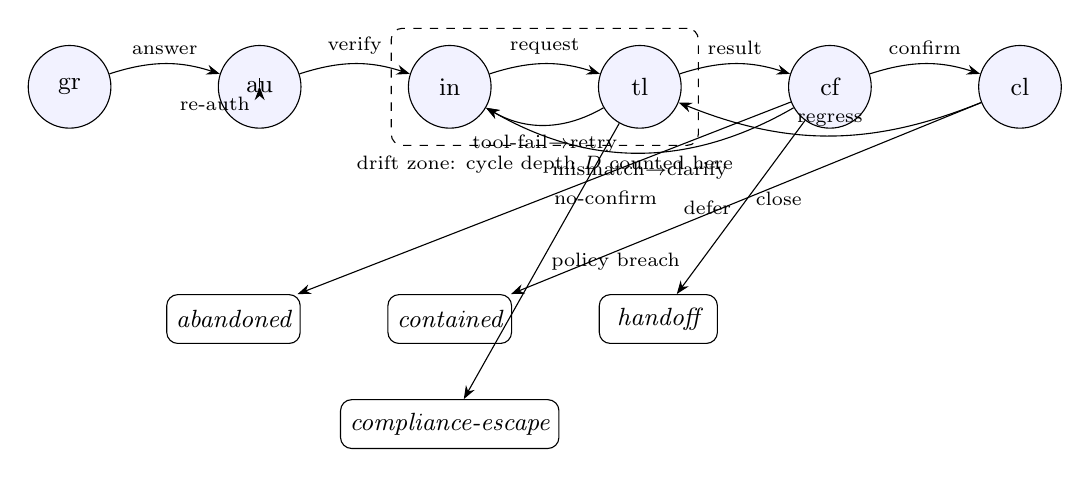
\begin{tikzpicture}[
  node distance=1.15cm and 1.35cm,
  state/.style={circle, draw, minimum size=1.05cm, font=\small, fill=blue!5},
  terminal/.style={rectangle, rounded corners, draw, minimum width=1.5cm, minimum height=0.62cm, font=\small\itshape},
  every edge/.append style={-Stealth, font=\scriptsize},
  looplabel/.style={font=\scriptsize, align=center},
]
\node[state] (gr) {gr};
\node[state, right=of gr] (au) {au};
\node[state, right=of au] (in) {in};
\node[state, right=of in] (tl) {tl};
\node[state, right=of tl] (cl) {cf};
\node[state, right=of cl] (co) {cl};

\node[terminal, below=2.1cm of in] (cont) {contained};
\node[terminal, left=1.1cm of cont] (aban) {abandoned};
\node[terminal, right=1.1cm of cont] (hand) {handoff};
\node[terminal, below=0.7cm of cont] (comp) {compliance-escape};

\draw (gr) edge[bend left=18] node[above]{answer} (au);
\draw (au) edge[bend left=18] node[above]{verify} (in);
\draw (in) edge[bend left=18] node[above]{request} (tl);
\draw (tl) edge[bend left=18] node[above]{result} (cl);
\draw (cl) edge[bend left=18] node[above]{confirm} (co);
\draw (co) edge node[right]{close} (cont);

% regression (cycle) edges
\draw (tl) edge[bend left=30] node[looplabel, below]{tool-fail$\to$retry} (in);
\draw (cl) edge[bend left=30] node[looplabel, below]{mismatch$\to$clarify} (in);
\draw (au) edge[bend right=35, looseness=1.4] node[looplabel, below left]{re-auth} (au);
\draw (co) edge[bend left=22] node[looplabel, above, sloped]{regress} (tl);

% terminal edges
\draw (cl) edge node[right]{no-confirm} (aban);
\draw (cl) edge node[left]{defer} (hand);
\draw (tl) edge node[looplabel, right]{policy breach} (comp);

% drift annotations
\begin{scope}[on background layer]
  \node[fit=(in)(tl), draw, dashed, rounded corners, inner sep=6pt, label={[font=\scriptsize]below:drift zone: cycle depth $D$ counted here}] {};
\end{scope}
\end{tikzpicture}%
  }
  \caption{The trajectory grammar $G$.
           Progress states (rounded) form the service spine; typed transitions ( labelled
           arrows) carry the eight event classes of Table~\ref{tab:transitions};
           regression types open cycles back into earlier states;
           terminal classes (squares) absorb every well-formed run.}
  \label{fig:grammar}
\end{figure}

The seven progress states cover the lifecycle of a banking call: identification, authentication,
intent capture, tool execution, clarification, confirmation, and closing.
The terminal classes are not generic success labels but the four production KPIs of conversational
banking: containment rate, abandonment rate, handoff rate, and compliance-escape rate.
Each class has an operational definition in telephony terms.
$\theta_{cont}$ (contained) holds when the run reaches a terminal through $q_{close}$ after a
confirmed service goal.
$\theta_{aban}$ (abandoned) holds when the caller disconnects before any terminal confirmation,
which in production surfaces as a hang-up event.
$\theta_{hand}$ (handoff) holds when an \texttt{escalation} transition fires, transferring the
caller to a human teller.
$\theta_{esc}$ (compliance-escape) holds when the run reaches a terminal confirmation without the
guarded \texttt{disclosure} transition having fired, which is precisely the false-success pattern
reported for tool agents \citep{falsesuccess2026}.
Industrial practice measures these quantities post hoc from telephony telemetry
\citep{nubank2026,silentabandonment2024}; under the grammar they become properties of runs.
This matters because final labels themselves mislead: agents can assert success while the task
failed \citep{falsesuccess2026}, so a terminal class must be derivable from the event stream
rather than from the agent's own closing statement.

\begin{table}[t]
\centering
\caption{Typed transitions of the trajectory grammar.
         Emitters are production components; regression types increment cycle depth.}
\label{tab:transitions}
\small
\begin{tabular}{lllll}
\toprule
Type & Direction & Source $\to$ Target & Emitter & Class \\
\midrule
\texttt{user-answer}   & progress   & $q_{auth/intent/clarify/confirm} \to$ next spine state & orchestrator LM      & dialogue \\
\texttt{agent-clarify} & either     & $q_{intent/confirm} \leftrightarrow q_{clarify}$       & orchestrator LM      & dialogue \\
\texttt{tool-call}     & progress   & $q_{tool} \to q_{tool}$ (iteration)                    & orchestrator         & system \\
\texttt{tool-fail}     & regression & $q_{tool} \to q_{tool}$ (retry)                        & backend tool         & system \\
\texttt{endpoint-error}& regression & $q_{intent/confirm} \to q_{intent}$                    & ASR endpointer       & voice \\
\texttt{user-bargein}  & event      & any $q_p \to q_p$ (audio channel)                      & barge-in detector    & voice \\
\texttt{disclosure}    & progress   & $q_{confirm} \to q_{close}$ (guarded)                  & compliance layer     & compliance \\
\texttt{escalation}    & progress   & any $q_p \to \theta_{hand}$                            & policy layer         & dialogue \\
\bottomrule
\end{tabular}
\end{table}

Table~\ref{tab:transitions} assigns every transition type to the component that emits it, which
is what makes the grammar checkable from telemetry: no state requires human annotation to
identify.
Two transition types are voice-physics events rather than dialogue acts: \texttt{endpoint-error}
fires when the endpointer commits a turn boundary too early or too late, and \texttt{user-bargein}
fires when the caller talks over the agent.
Both are observable from the same detection stages that bound response onset and cessation in the
published floors \citep{garcia2026latencyfloor,garcia2026cessationfloor}.
The \texttt{agent-clarify} type is marked \emph{either} because a clarification is progress when
it resolves an ambiguity and a regression when it re-opens a settled state; the grammar does not
prejudge which, and the cycle count of Definition~\ref{def:cycledepth} is what decides.
The \texttt{user-bargein} type leaves the state unchanged because a barge-in is a channel event,
not a conversation state; its conversational meaning is an observation for the posterior of
Definition~\ref{def:posterior}, not a state change.
This separation keeps the grammar auditable: every state change has a named emitter in the
orchestration stack, and channel events never mutate conversation state by themselves.

\begin{definition}[Run]
\label{def:run}
A \emph{run} of $G$ is a finite alternating sequence
$\sigma = q_0\, t_1\, q_1\, \cdots\, t_n\, q_n$ with $q_0 = q_{greet}$, $q_n \in T$, and each
$(t_i, q_i)$ permitted by $\delta$.
A \emph{partial run} is any proper prefix $\sigma_{\leq j}$ of a well-formed run that ends in a
non-terminal state.
The \emph{true outcome} of $\sigma_{\leq j}$ is the terminal class of the well-formed run that
extends it, which is unique by absorption but unobserved while the conversation runs.
Early outcome prediction is exactly the problem of guessing this unobserved terminal class from
$\sigma_{\leq j}$, and Section~4 states when that guess may be acted on.
$\sigma$ is \emph{well-formed} if every terminal class is absorbing, i.e., no transition departs
from a state in $T$.
Well-formedness is a safety property of the orchestration policy, not of the data: a run that
continues after a terminal class is a policy bug, and the grammar makes such bugs detectable by
inspection of $\delta$.
\end{definition}

\subsection{Cycles and the Drift Statistic}

\begin{definition}[Cycle and cycle depth]
\label{def:cycledepth}
A \emph{cycle} of a run $\sigma$ is a maximal sub-run that departs from a state $q$ and later
returns to $q$, where $q$ is non-terminal.
The \emph{cycle depth} $D(\sigma)$ is the number of cycles in $\sigma$.
\end{definition}

The intuition is operational: one clarification after a failed balance lookup is normal service,
whereas a third return to $q_{clarify}$ is a conversation going in circles.
Cycle depth turns this intuition into a countable statistic that separates two failure modes that
conversation-length measures conflate.
Three properties fix the statistic's behaviour.
First, $D(\sigma)$ counts returns, not repetitions: iterating \texttt{tool-call} inside
$q_{tool}$ is spine progress, while returning to $q_{intent}$ after having confirmed is drift.
Second, $D$ is monotone along a run, so the monitor maintains it online at zero detection cost
beyond event counting.
Third, $D$ is defined identically for real and simulated runs, which makes it portable to the
protocols of \citet{sierra2024taubench} and the workflow corpora of
\citet{salesforce2025workflows} without re-labelling.

\begin{proposition}[Longer is not off-path]
\label{prop:longer_offpath}
There exist well-formed runs $\sigma_L$ and $\sigma_D$ of equal length $n$ with
$D(\sigma_L) = 0$ and $D(\sigma_D) \geq 1$.
Hence run length alone determines neither drift nor the terminal class, and any outcome detector
keyed to conversation duration confuses the two.
The distinction has direct operational value: a long call that is merely tool-heavy should not
page a supervisor, while a short call with two clarification cycles may already be failing.
\end{proposition}

\begin{proof}
Construct $\sigma_L$ as the direct spine
$q_{greet} \to q_{auth} \to q_{intent} \to q_{tool} \to q_{confirm} \to q_{close} \to \theta_{cont}$
padded with $n - 6$ \texttt{tool-call} iterations inside $q_{tool}$; no state is departed and
revisited, so $D(\sigma_L) = 0$.
Construct $\sigma_D$ with the same number of transitions but routing two of them through
$q_{confirm} \to q_{clarify} \to q_{confirm}$ via \texttt{agent-clarify}, removing an equal number
of \texttt{tool-call} iterations to hold length fixed; this sub-run departs from and returns to
$q_{confirm}$, so $D(\sigma_D) \geq 1$.
Both runs are well-formed and of length $n$, which proves the claim.
\end{proof}

\begin{figure}[t]
  \centering
  \resizebox{\linewidth}{!}{%
    % fig_cycles.tex — contained vs drifted trajectories as grammar walks (cycle depth)
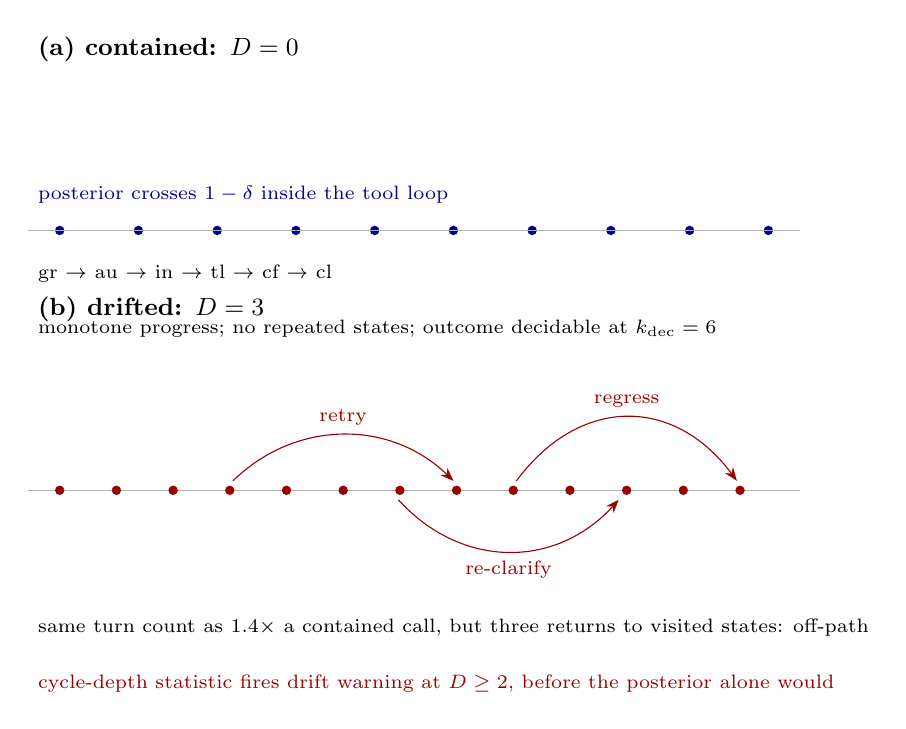
\begin{tikzpicture}[xscale=1.0, yscale=1.0]
% Panel A: contained call (low cycle depth)
\begin{scope}
  \node[font=\small\bfseries, anchor=west] at (-0.4,2.3) {(a) contained: $D=0$};
  % turn dots along a line
  \foreach \i in {0,...,9} { \fill[blue!60!black] (\i,0) circle (1.7pt); }
  \draw[gray!60] (-0.4,0) -- (9.4,0);
  % state strip
  \node[font=\scriptsize, anchor=west] at (-0.4,-0.55) {gr $\to$ au $\to$ in $\to$ tl $\to$ cf $\to$ cl};
  \node[font=\scriptsize, align=left, anchor=west] at (-0.4,-1.25) {monotone progress; no repeated states; outcome decidable at $k_{\mathrm{dec}}=6$};
  \node[font=\scriptsize, blue!60!black, anchor=west] at (-0.4,0.45) {posterior crosses $1-\delta$ inside the tool loop};
\end{scope}
% Panel B: drifted call (high cycle depth)
\begin{scope}[yshift=-3.3cm]
  \node[font=\small\bfseries, anchor=west] at (-0.4,2.3) {(b) drifted: $D=3$};
  \draw[gray!60] (-0.4,0) -- (9.4,0);
  \foreach \i in {0,...,12} { \fill[red!60!black] (\i*0.72,0) circle (1.7pt); }
  % cycles drawn as arcs back
  \draw[-Stealth, red!60!black] (2.2,0.12) .. controls (3.0,0.9) and (4.2,0.9) .. (5.0,0.12)
    node[midway, above, font=\scriptsize] {retry};
  \draw[-Stealth, red!60!black] (4.3,-0.12) .. controls (5.1,-1.0) and (6.3,-1.0) .. (7.1,-0.12)
    node[midway, below, font=\scriptsize] {re-clarify};
  \draw[-Stealth, red!60!black] (5.8,0.12) .. controls (6.6,1.2) and (7.8,1.2) .. (8.6,0.12)
    node[midway, above, font=\scriptsize] {regress};
  \node[font=\scriptsize, align=left, anchor=west] at (-0.4,-1.75) {same turn count as 1.4$\times$ a contained call, but three returns to visited states: off-path};
  \node[font=\scriptsize, red!60!black, anchor=west] at (-0.4,-2.45) {cycle-depth statistic fires drift warning at $D\geq 2$, before the posterior alone would};
\end{scope}
\end{tikzpicture}%
  }
  \caption{Cycle depth as drift.
           Two runs of equal length: the contained run (top) iterates \texttt{tool-call} within
           $q_{tool}$ and stays on the spine; the drifted run (bottom) opens a
           $q_{confirm} \to q_{clarify} \to q_{confirm}$ cycle.
           Length is identical; only cycle depth distinguishes them.}
  \label{fig:cycles}
\end{figure}

Cycle depth would be unbounded without a turn-scale trigger, and the published latency program
supplies one.

\begin{lemma}[Cycle-length bound]
\label{lem:cyclebound}
Fix a per-response deadline $\tau_{resp}$ and the latency parameters of the cascade pipeline, and
let $\Lambda_k = \lambda_{asr} + k \cdot \lambda_{lm} + (k-1) \cdot \lambda_{tool} + \lambda_{tts}$
be the $k$-step silence gap of \citet{garcia2026latencyfloor}.
Let $k^* = \max\{k : \Lambda_k \leq \tau_{resp}\}$.
Then:
(i) any run segment between two consecutive user turns that emits more than $k^*$
\texttt{tool-call} transitions violates the response deadline, and is therefore off-path for every
deadline-conforming policy;
(ii) under the patience-hazard model of \citet{silentabandonment2024}, the probability that the
caller remains on the line decays with each deadline breach, so runs far beyond $k^*$ terminate
in $\theta_{aban}$ with high probability.
\end{lemma}

\begin{proof}
For (i), each \texttt{tool-call} iteration inside one orchestrated turn adds one LM step and one
tool round-trip to the user-perceived silence gap, which grows linearly in $k$ by the compounding
result of \citet{garcia2026latencyfloor}; emitting more than $k^*$ such transitions therefore
produces a silence gap exceeding $\tau_{resp}$, which no deadline-conforming policy permits.
For (ii), each breached deadline raises the instantaneous hang-up hazard estimated from
contact-center patience data \citep{silentabandonment2024}; iterating the hazard over repeated
breaches drives the survival probability to zero, which yields the high-probability claim.
\end{proof}

\begin{remark}
\label{rem:drift_trigger}
Lemma~\ref{lem:cyclebound} makes drift detection an event-counting rule, not a timeout: the
monitor raises a drift alarm at the $(k^*{+}1)$-th \texttt{tool-call} event, in real time and
without waiting for the response to complete.
Because \texttt{tool-call} events are emitted by the orchestrator itself, the count is exact; the
only probabilistic component is the caller-patience channel in claim (ii).
The alarm's own detection latency is the monitor's decision time, which Section~4 bounds by a
stopping rule and Section~5 accounts against the published floors.
Two properties make $k^*$ usable in production rather than merely in theory.
It is monotone in the deadline: relaxing $\tau_{resp}$ raises $k^*$, so the drift trigger adapts
to policy rather than being hard-coded.
And it is auditable: given the latency table of the deployed cascade, $k^*$ is a one-line
computation that a reviewer can re-derive from the floor arithmetic of
\citet{garcia2026latencyfloor} alone.
\end{remark}

\subsection{Multi-Channel Observation Model}

\begin{definition}[Observation]
\label{def:observation}
At turn $k$ the monitor observes the tuple
$o_k = (x_k, s_k, e_k, f_k)$:
the partial transcript $x_{1:k}$;
the turn-state sequence $s_{1:k}$ labelling each utterance as completion, backchannel, or
interruption \citep{x2turn2026};
the tool-event log $e_{1:k}$ emitted by the orchestrator; and
the acoustic flags $f_{1:k}$ recording endpointing errors and barge-ins
\citep{garcia2026cessationfloor}.
Every channel is streaming: each component updates incrementally, so $o_k$ is available within one
turn of real time and no channel requires the conversation to have ended.
\end{definition}

The channels are not interchangeable, and the transcript channel is the weakest one.
Text-only turn-end decisions sit near chance on Spanish hard cuts (accuracy $0.40$--$0.54$), as
measured in our semantic-VAD study \citep{garcia2026asking}; a grammar that conditioned only on
$x_{1:k}$ would therefore inherit that blindness at conversation scale.
The turn-state and tool-event channels carry exactly the information the text channel lacks:
$s_k$ distinguishes completed intents from backchannels, and $e_k$ reports system-side progress
that never surfaces in the transcript at all.

\begin{definition}[Outcome posterior]
\label{def:posterior}
Given the observation history $o_{1:k}$, the outcome posterior is
$p(\theta \mid o_{1:k})$ over terminal classes $\theta \in T$.
\end{definition}

The posterior is defined to be recomputable after every event, not only at turn boundaries,
because every channel updates incrementally in a streaming cascade.
Section~4 places a sequential stopping rule over $p(\theta \mid o_{1:k})$ and derives when the
monitor may act on it.
The price of early warning is paid per turn inside the same floor arithmetic as the response
itself: the published cloud decision latencies (p99 $178$--$268$~ms) \citep{garcia2026asking}
bound what each posterior update adds, and every intervention triggered by the posterior must
additionally clear the cessation floor before the agent's audio actually stops
\citep{garcia2026cessationfloor}.


\section{Stopping Rules for Outcome Prediction}
\label{sec:stopping}
% §4 Stopping Rules for Outcome Prediction
The grammar of Section~\ref{sec:grammar} turns a conversation into a walk over $Q$ that emits typed observations at every turn.
A decision layer must convert this growing evidence into an action --- intervene, escalate, flag, or wait --- at a time that is early enough to matter and honest about its own error rates.
This section defines that layer: an outcome-class posterior maintained per turn, a sequential stopping rule over the posterior, and cost-asymmetric decision boundaries derived from the banking cost model.
The centerpiece is the Trajectory Stopping Theorem, which bounds the expected decision time at a prescribed confidence and subsumes the fixed-threshold triggering of learned early-failure detectors as a special case.

\subsection{From Grammar Emissions to an Outcome Posterior}
\label{subsec:posterior}
At turn $k$ the monitor observes the multi-channel tuple $o_k$ of Definition~\ref{def:observation}: the partial transcript, the turn-state sequence, the tool-event log, and the acoustic flags.
Together these channels induce the outcome-class posterior $p(\theta \mid o_{1:k})$ over the terminal set $T = \{\theta_{cont}, \theta_{aban}, \theta_{hand}, \theta_{esc}\}$.
The posterior is deliberately abstract: any calibrated estimator over grammar emissions suffices, and every guarantee below attaches to the stopping layer rather than to a particular model.
That partial trajectories carry outcome signal at all is established for offline evaluation pruning \citep{earlyeval2026} and for text-chat failure forecasting \citep{nourbakhsh2026tracer}; our contribution is a live decision layer with guarantees, not another estimator.
Two design constraints come from our published results rather than from new evidence.
First, text-only turn signals are near chance on Spanish hard cuts \citep{garcia2026asking}, so the posterior must condition on the multi-channel observation $o_{1:k}$, not on the transcript alone.
Second, the cycle depth $D(\sigma)$ of the grammar is its drift statistic, and it enters the posterior as a covariate: each regression transition shifts probability mass toward the action classes.
Deep tool episodes are precisely where banking conversations drift, and the $k$-step analysis of cascade agents makes the cost of such episodes formal \citep{garcia2026latencyfloor}.

\subsection{Sequential Stopping over the Posterior}
\label{subsec:rule}
The sequential probability ratio test (SPRT) is the canonical likelihood-ratio procedure with type-I and type-II error control \citep{wald1947sprt}, recently transposed to early-stopping of LLM reasoning paths \citep{consol2025}.
We transpose it once more, from reasoning paths to conversation turns.

\begin{definition}[Sequential outcome decision rule]
\label{def:rule}
Fix the benign class $\theta_0 = \theta_{cont}$ and, for each action class $\theta_a \in T \setminus \{\theta_0\}$, let
\begin{equation}
  \label{eq:llr}
  \ell_k^{a} \;=\; \log \frac{p(o_{1:k} \mid \theta_a)}{p(o_{1:k} \mid \theta_0)}
\end{equation}
denote the log-likelihood ratio of the observed emission stream under $\theta_a$ versus $\theta_0$.
With target false-alarm rate $\alpha_a$ and miss rate $\beta_a$ for class $\theta_a$, set the upper and lower boundaries
\begin{equation}
  \label{eq:boundaries}
  A_a = \log \frac{1}{\alpha_a}, \qquad B_a = \log \beta_a .
\end{equation}
The decision time is
\begin{equation}
  \label{eq:kdec}
  k_{\mathrm{dec}} \;=\; \min\Bigl(\;
    \min\{k : \exists\, a,\; \ell_k^{a} \geq A_a \;\text{(declare } \theta_a)\},\;\;
    \min\{k : \forall\, a,\; \ell_k^{a} \leq B_a \;\text{(declare } \theta_0)\},\;\;
    k_{\mathrm{term}}
  \Bigr),
\end{equation}
where $k_{\mathrm{term}}$ is the turn at which the grammar walk reaches a terminal state and the outcome is observed directly.
\end{definition}

The rule is one-sided per action class and jointly conservative: declaring \emph{no action} requires every class-wise ratio to fall below its lower boundary, so a conversation cannot be written off as contained while any action hypothesis retains evidence.
This asymmetry is deliberate and is priced in Section~\ref{subsec:economics}.
The boundary form \eqref{eq:boundaries} is the Ville-style parametrisation rather than the classical Wald form $\log\frac{1-\beta}{\alpha}$: because the rule monitors each class ratio past its own lower boundary (another class may still be above its $B$), the operative error event for declaring $\theta_a$ under $\theta_0$ is \emph{ever crossing} $A_a$, and Ville's inequality prices exactly that event, at the cost of slightly wider boundaries than the two-sided classical SPRT.

\subsection{The Trajectory Stopping Theorem}
\label{subsec:theorem}
We now state the guarantee.
The assumptions are explicit because each is load-bearing.
(i) \emph{Correct specification}: the emission densities used in \eqref{eq:llr} coincide with the true data-generating densities given the terminal class.
(ii) \emph{Increment separation}: emissions are conditionally independent given the terminal class, the per-turn log-ratio increments are integrable and bounded, $|Z_k^{a}| \leq c$ for a known constant $c$, and their conditional means are strictly separated: under $\theta_a$ at least $\mu_1^{a} > 0$, and under $\theta_0$ at most $\mu_0^{a} < 0$, for every action class $a$.
(iii) \emph{Termination}: the grammar walk reaches a terminal state in bounded expected time, $\mathbb{E}[k_{\mathrm{term}}] < \infty$; this is a property of the orchestration policy (Definition~\ref{def:run} makes non-terminating runs a policy bug), not of the theorem --- note that the \texttt{tool-call} self-loop makes unbounded runs representable, so the assumption must be checked against the deployed policy.

\begin{theorem}[Trajectory Stopping]
\label{thm:stopping}
Under conditions (i)--(iii), the decision rule of Definition~\ref{def:rule} satisfies, for every action class $a$:
\begin{align}
  \Pr\bigl[\text{declare } \theta_a \mid \theta_0\bigr] &\leq \alpha_a,
  &
  \Pr\bigl[\text{declare } \theta_0 \mid \theta_a\bigr] &\leq \beta_a,
  \label{eq:errors}\\
  \mathbb{E}\bigl[k_{\mathrm{dec}} \mid \theta_a\bigr]
    &\leq \frac{A_a + c}{\mu_1^{a}},
  &
  \mathbb{E}\bigl[k_{\mathrm{dec}} \mid \theta_0\bigr]
    &\leq \min\Biggl(\mathbb{E}\bigl[k_{\mathrm{term}}\bigr],\;
      \sum_{j \in A} \frac{|B_j| + c}{|\mu_0^{\,j}|}\Biggr),
  \label{eq:times}
\end{align}
where $A = T \setminus \{\theta_0\}$ is the action-class set.
The $\theta_0$-side bound aggregates over classes because declaring \emph{no action} requires
\emph{every} class-wise ratio to fall below its own lower boundary (Definition~\ref{def:rule}),
so $k_{\mathrm{dec}}$ under $\theta_0$ is gated by the slowest class-wise descent, not by any
single class.
Consequently, for any prior $\pi$ over $T$,
\begin{align}
  \label{eq:unconditional}
  \mathbb{E}[k_{\mathrm{dec}}] \;=\; \textstyle\sum_{\theta \in T} \pi_\theta\, \mathbb{E}[k_{\mathrm{dec}} \mid \theta] \;\leq\; K(\varepsilon, c),
\\[2pt]
  K(\varepsilon, c) \;:=\; \max\Biggl(\max_{a \in A} \tfrac{A_a + c}{\mu_1^{a}},\;
  \min\bigl(\mathbb{E}[k_{\mathrm{term}}], \textstyle\sum_{j \in A} \tfrac{|B_j| + c}{|\mu_0^{\,j}|}\bigr)\Biggr),
\end{align}
and by the union bound the error probability against the budgeted error events obeys
$\varepsilon := \sum_{a} (\alpha_a + \beta_a)$, so decisions are delivered in at most
$K(\varepsilon, c)$ expected turns at confidence at least $1 - \varepsilon$ against those events,
under a calibrated emission model.
A remark on the frontier: as $\beta_{esc} \to 0$ under the cost ordering of Proposition~\ref{prop:asymmetric}, $|B_{esc}|$ inflates the $\theta_0$-side sum in \eqref{eq:times} --- the price of "contained must be earned" is a slower earned verdict, an inherent SPRT trade-off the protocol measures rather than hides.
\end{theorem}

\begin{proof}[Proof sketch]
Fix an action class $a$.
Under $\theta_0$ and correct specification, the likelihood ratio of the emissions makes
$\exp(\ell_k^{a})$ a mean-one non-negative martingale: conditional independence is not needed
here, only that $\exp(\ell_k^{a})$ is the density ratio of the true conditional law, so
$\mathbb{E}_{\theta_0}[e^{Z_k^{a}} \mid \mathcal{F}_{k-1}] = 1$ exactly.
Ville's inequality then prices the ever-crossing event directly:
$\Pr_{\theta_0}[\exists k \leq k_{\mathrm{term}}: \ell_k^{a} \geq A_a] \leq e^{-A_a} = \alpha_a$,
which is the first bound of \eqref{eq:errors}; the second follows symmetrically by applying
Ville's inequality to $\exp(-\ell_k^{a})$ under $\theta_a$, whose crossing level $-B_a$ yields
$e^{B_a} = \beta_a$.
For the $\theta_a$-side time bound, use $a$'s \emph{own} upper crossing as the envelope: on the
event that $a$ is declared, $k_{\mathrm{dec}}$ is at most the first time $\ell_k^{a}$ reaches
$A_a$, and Wald's first identity (which presupposes $\mathbb{E}[k_{\mathrm{dec}}] < \infty$;
truncating at $k_{\mathrm{term}}$ and passing to the limit discharges this under assumption (iii))
gives $\mathbb{E}[\ell_k^{a} \wedge A_a] \leq A_a + c$ after $\lceil (A_a+c)/\mu_1^{a} \rceil$
turns in expectation, with Lorden-type overshoot bounds keeping the excess within $c$
\citep{lorden1970excess}.
Under $\theta_0$, declaring $\theta_0$ requires all $|A|$ ratios to descend below their $B_j$;
the expected time for the slowest descent is bounded by the sum of the per-class expected
descent times, $\sum_j (|B_j| + c)/|\mu_0^{\,j}|$, and the observed-termination mode is bounded
by $\mathbb{E}[k_{\mathrm{term}}]$ via assumption (iii), giving the second display of
\eqref{eq:times}.
The unconditional bound \eqref{eq:unconditional} takes the max of the conditional envelopes,
and the error budget is the union bound over the per-class error events
\eqref{eq:errors}.
\end{proof}

\begin{remark}[What the budget prices]
\label{rem:budget_scope}
The budget $\varepsilon = \sum_a (\alpha_a + \beta_a)$ prices two error families: declaring an
action class under the benign truth ($\theta_a \mid \theta_0$) and writing the conversation off
under an action truth ($\theta_0 \mid \theta_a$).
It does not price \emph{cross-action} misdeclarations (declaring $\theta_b$ when the truth is
$\theta_a$, $b \neq a$): $e^{\ell^b}$ is not a martingale under $\theta_a$, so Ville on
$\ell^b$ alone says nothing there; the pairwise likelihood-ratio martingale $e^{\ell^b - \ell^a}$
gives $\Pr_{\theta_a}[\text{declare } \theta_b] \leq \alpha_b / \alpha_a$ when $A_b > A_a$.
Since handoff-versus-escape confusion is economically real (Section~\ref{subsec:economics}), a
deployment that must price it adds pairwise boundaries on $\ell^a - \ell^j$ with a per-pair
budget; we leave that extension to the protocol of Section~\ref{sec:evaluation} as an operating
curve, not a theorem.
\end{remark}

Three remarks on what the theorem does and does not say.
First, the assumption we cannot discharge is per-turn conditional independence of emissions; it holds to the extent that the grammar's typed transitions, not hidden user state, drive the observation stream, and Section~\ref{sec:discussion} returns to this.
Second, the $c$ terms are the standard excess-over-boundary (overshoot) constants; in the idealised continuous treatment they vanish, and as design guidance they are one turn at most (the protocol of Section~
ef{sec:evaluation} measures them), which is why \eqref{eq:times} is displayed with them explicit rather than hidden.
Third, where the emission likelihood is unknown and the posterior is learned, likelihood ratios are unavailable in exact form.
The honest sequential alternative is an anytime-valid confidence sequence over the learned posterior, which retains error control under continuous monitoring and optional stopping \citep{howard2021time} at the price of wider early boundaries; we adopt this variant in the evaluation protocol of Section~\ref{sec:evaluation} and report both operating curves.
Wald-type SPRT remains the reference point because its boundaries are explicit and its expected stopping time is optimal among two-hypothesis tests with the same error rates \citep{waldwolfowitz1948optimality}; that optimality is a property of the classical two-sided test, not of the wider-boundary three-exit rule deployed here.

\begin{figure}[t]
  \centering
  \resizebox{\linewidth}{!}{%
    % fig_stopping.tex — stopping rule timeline over the outcome-class posterior
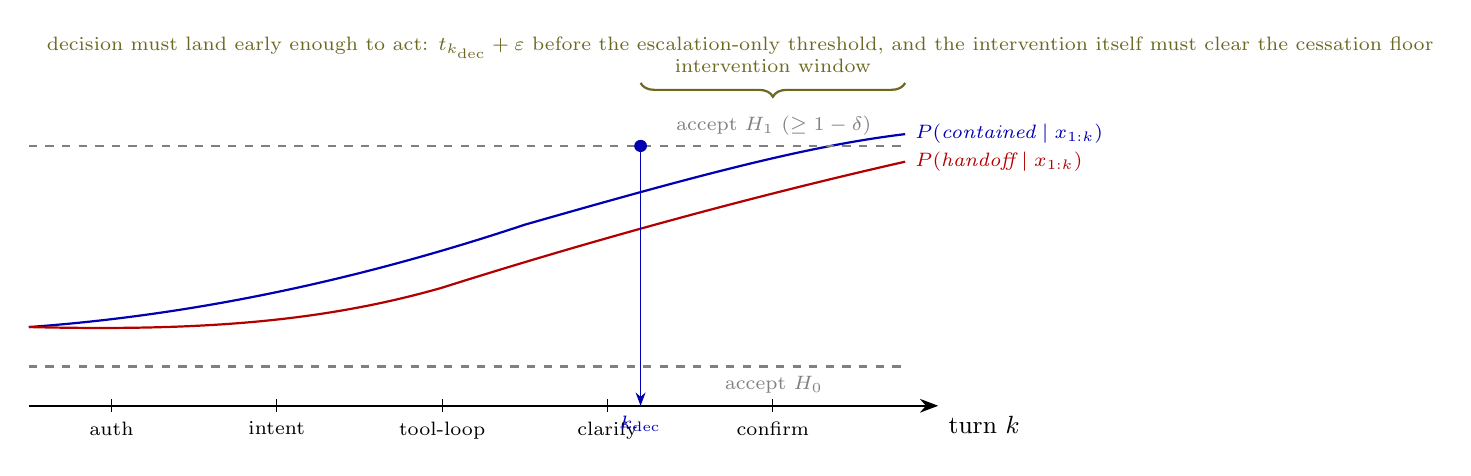
\begin{tikzpicture}[xscale=1.05, yscale=1.0]
% time axis: turns
\draw[-Stealth, thick] (0,0) -- (11,0) node[below right, font=\small] {turn $k$};
\foreach \k/\lbl in {1/{auth}, 3/{intent}, 5/{tool-loop}, 7/{clarify}, 9/{confirm}} {
  \draw (\k,0.08) -- (\k,-0.08) node[below, font=\scriptsize] {\lbl};
}
% posterior curves (stylized) for two classes
\draw[thick, blue!70!black] (0,1.0) .. controls (2,1.15) and (4,1.6) .. (6,2.3)
  .. controls (8,2.9) and (9.4,3.3) .. (10.6,3.45)
  node[right, font=\scriptsize, blue!70!black] {$P(\textit{contained}\mid x_{1:k})$};
\draw[thick, red!70!black] (0,1.0) .. controls (2,0.95) and (3.5,1.05) .. (5,1.5)
  .. controls (6.5,2.0) and (8.5,2.6) .. (10.6,3.1)
  node[right, font=\scriptsize, red!70!black] {$P(\textit{handoff}\mid x_{1:k})$};
% SPRT boundaries
\draw[dashed, thick, gray] (0,3.3) -- (10.6,3.3) node[above, font=\scriptsize, pos=0.85] {accept $H_1$ ($\geq 1-\delta$)};
\draw[dashed, thick, gray] (0,0.5) -- (10.6,0.5) node[below, font=\scriptsize, pos=0.85] {accept $H_0$};
% crossing point: contained class crosses upper boundary at k*
\fill[blue!70!black] (7.4,3.3) circle (2.2pt);
\draw[-Stealth, blue!70!black] (7.4,3.3) -- (7.4,0) node[below, font=\scriptsize, blue!70!black] {$k_{\mathrm{dec}}$};
% intervention window vs escalation-only threshold
\draw[decorate, decoration={brace, mirror, amplitude=5pt}, thick, olive!70!black] (7.4,4.1) -- (10.6,4.1)
  node[midway, above, font=\scriptsize, olive!70!black] {intervention window};
\node[font=\scriptsize, olive!70!black, align=left, anchor=west] at (0.1,4.55)
  {decision must land early enough to act: $t_{k_{\mathrm{dec}}} + \varepsilon$ before the escalation-only threshold, and the intervention itself must clear the cessation floor};
\end{tikzpicture}%
  }
  \caption{The stopping layer over a live conversation.
           Class-wise log-likelihood ratios $\ell_k^{a}$ accumulate with their boundary pair
           $(B_a, A_a)$; the first upper crossing declares an action class and fires an
           intervention whose decision latency $\lambda_{\mathrm{decide}}$ and cessation
           latency $\lambda_{\mathrm{cease}}$ must both fit inside the remaining window
           before the escalation-only threshold.}
  \label{fig:stopping}
\end{figure}

\subsection{Floor Composition: Early Enough to Act}
\label{subsec:floors}
A turn index is not an intervention guarantee, so we convert $k_{\mathrm{dec}}$ to wall-clock using the published floor arithmetic.
The per-turn decision latency $\lambda_{\mathrm{decide}}$ of the monitor must fit inside the inter-turn budget that the onset floor leaves unfilled \citep{garcia2026latencyfloor}, and the measured decision latencies of the Spanish interim-transcript pipeline (p99 178--268~ms, cloud) show this budget exists in production \citep{garcia2026asking}.
Executing the intervention is a second bound: taking the floor from an agent mid-utterance is a barge-in, and it must clear the cessation floor's detect--decide--cease--resume decomposition \citep{garcia2026cessationfloor}.
The composition is therefore
\begin{equation}
  \label{eq:compose}
  t_{k_{\mathrm{dec}}} + \lambda_{\mathrm{decide}} + \lambda_{\mathrm{cease}}
  \;<\;
  t_{\mathrm{escalation\text{-}only}},
\end{equation}
and only conversations satisfying \eqref{eq:compose} are ones where early prediction converts into an actionable intervention rather than a post-hoc annotation.
The cycle-length bound of Section~\ref{sec:grammar} completes the picture from the other side: a run segment exceeding $k_{\mathrm{cyc}}$ \texttt{tool-call} iterations violates the response deadline, so the stopping rule rarely has to wait past the horizon the grammar already justifies.

\subsection{False-Early-Exit Economics}
\label{subsec:economics}
Stopping early is only justified if the cost model says so.
Let $c(\hat{\theta}, \theta)$ denote the banking cost of declaring class $\hat{\theta}$ when the truth is $\theta$, over declared versus true terminal classes; its operational content is specified with the KPI wiring of Section~\ref{sec:evaluation}.
False containment --- declaring \textit{contained} while the truth is \textit{handoff} or \textit{compliance-escape} --- is the expensive error: it converts a recoverable failure into an unattended one, and a compliance escape has unbounded cost.
False escalation --- declaring \textit{handoff} while the truth is \textit{contained} --- wastes teller minutes, the trade that queue-level control already prices from the outside of the conversation \citep{queuecontrol2026}.
Abandonment adds a patience-driven cost that queueing models estimate from uncertain data \citep{silentabandonment2024}; the grammar lets us price it from the conversation's own trajectory.

\begin{proposition}[Cost-asymmetric boundaries]
\label{prop:asymmetric}
Let the cost model satisfy $c(\theta_0, \theta_a) > c(\theta_a, \theta_0)$ for every action class $a$, with $c(\theta_0, \theta_{esc})$ unbounded.
Then the Bayes-optimal single-turn threshold for declaring $\theta_{esc}$ tends to zero, so the compliance boundary fires at the first credible signal: $\alpha_{esc}$ is elevated, $A_{esc} = \log(1/\alpha_{esc})$ is the smallest upper boundary, and $\beta_{esc}$ tends to zero.
Between the remaining action classes, larger relative miss cost $c(\theta_0, \theta_a)/c(\theta_a, \theta_0)$ yields a smaller threshold, hence a smaller $A_a$ and a larger $\alpha_a$.
\end{proposition}

\begin{proof}[Proof sketch]
For a single-turn Bayes decision with posterior $p(\theta_a \mid o_{1:k})$, the optimal rule declares $\theta_a$ exactly when the posterior exceeds the cost ratio $\frac{c(\theta_a,\theta_0)}{c(\theta_a,\theta_0) + c(\theta_0,\theta_a)}$.
An unbounded $c(\theta_0, \theta_{esc})$ drives that ratio to zero, so the compliance escape fires at any positive posterior mass; in the Ville parametrisation \eqref{eq:boundaries} this is an elevated false-alarm rate $\alpha_{esc}$ and hence the smallest upper boundary $A_{esc}$, while the miss rate $\beta_{esc}$ --- the probability of declaring $\theta_0$ when the truth is $\theta_{esc}$ --- is driven to zero by the same eagerness.
Monotonicity in the relative miss cost follows from differentiating the threshold ratio.
The sequential rule inherits the ordering because its boundaries are the sequential realization of the same posterior-threshold test at every turn.
\end{proof}

The practical reading is that the four terminal classes do not share one threshold.
A banking monitor should fire its compliance escape at the first credible signal, accept a higher false-escape rate as the price of unbounded miss cost, and treat contained as a verdict that must be earned against every action hypothesis simultaneously.

\subsection{TRACER as the Fixed-Sample Instance}
\label{subsec:tracer}
The nearest published system to this decision layer is TRACER, which scores every visible dialogue prefix for eventual failure and fires a recovery trigger when the score exceeds a development-tuned threshold $\tau = 0.7788$, frozen under a false-positive-rate constraint of $0.15$ \citep{nourbakhsh2026tracer}.

\begin{corollary}[Fixed-sample instance]
\label{cor:tracer}
TRACER's thresholded trigger is the fixed-sample instance of Definition~\ref{def:rule}: a single look at each prefix with a learned posterior, a one-sided boundary in place of the pair \eqref{eq:boundaries}, and no optional stopping.
The Trajectory Stopping Theorem adds the three properties that a single-look trigger cannot express: an expected decision-time bound \eqref{eq:times}, error control that survives continuous monitoring (via the confidence-sequence variant of \citealp{howard2021time}), and cost-derived asymmetry across the four banking outcome classes instead of one binary failure label.
\end{corollary}

This is a generalization claim, not a criticism: TRACER's detected signals appear from the first quarter of the dialogue and its operating point is honest about its false-positive budget \citep{nourbakhsh2026tracer}.
What the sequential layer contributes is the freedom to stop looking, the price of that freedom in turns, and thresholds that differ per outcome class because the costs differ.
The evaluation protocol of Section~\ref{sec:evaluation} therefore uses TRACER's early-detection metrics with credit, extended with the cost-weighted decision-latency accounting that floor composition demands.


\section{A Banking KPI-Tuned Evaluation Protocol}
\label{sec:evaluation}
% §5 Contact-Centre KPI-Tuned Evaluation Protocol on Public Benchmarks
This section specifies how the trajectory grammar and the stopping rule are evaluated on public task-oriented dialogue benchmarks.
The protocol is tuned to contact-centre KPIs: every terminal class in the outcome set $T = \{\theta_{cont}, \theta_{aban}, \theta_{hand}, \theta_{esc}\}$ of Section~\ref{sec:grammar} --- contained, abandoned, handoff, compliance-escape --- is wired to a metric that a contact-centre operator already tracks.
Figure~\ref{fig:eval_stack} summarises the wiring from grammar states and terminal classes to contact-centre telemetry and per-turn decision signals.
All experimental evidence comes from public datasets; the KPI wiring below is the interface by which public outcome labels acquire operational meaning.

\begin{figure}[t]
  \centering
  \resizebox{\linewidth}{!}{%
    % fig_eval_stack.tex — banking KPI wiring: trajectory classes to telemetry and interventions
\begin{tikzpicture}[
  font=\small,
  box/.style={rectangle, rounded corners, draw, minimum height=0.75cm, inner sep=5pt, align=center},
  kpi/.style={box, fill=olive!8},
  layer/.style={box, fill=blue!6},
  act/.style={box, fill=red!6},
  every edge/.append style={-Stealth, font=\scriptsize},
  node distance=0.55cm and 0.8cm,
  
]
% sensing layer
\node[layer] (sens) {sensing: partial transcript + turn states + tool events + endpointing/barge-in flags};
% grammar layer
\node[layer, below=of sens] (gram) {trajectory grammar $G=(Q,\Sigma,\delta)$: state estimate + cycle depth $D$};
% stopping layer
\node[layer, below=of gram] (stop) {stopping rule over $P(\theta\mid x_{1:k})$: decide at $k_{\mathrm{dec}}\leq k^\ast$, confidence $1-\delta$};
% KPI classes
\node[kpi, below left=0.8cm and -1.2cm of stop] (cont) {contained};
\node[kpi, right=of cont] (aban) {abandoned};
\node[kpi, right=of aban] (hand) {handoff};
\node[kpi, right=of hand] (comp) {compliance-escape};
% interventions
\node[act, below=1.5cm of cont] (none) {continue (no action)};
\node[act, below=1.5cm of aban] (probe) {proactive clarification};
\node[act, below=1.5cm of hand] (esc) {warm transfer to teller};
\node[act, below=1.5cm of comp] (fraud) {fraud flag + policy route};

\draw (sens) -- (gram);
\draw (gram) -- (stop);
\draw (stop.south) -- ++(0,-0.35) -| (cont.north);
\draw (stop.south) -- ++(0,-0.35) -| (aban.north);
\draw (stop.south) -- ++(0,-0.35) -| (hand.north);
\draw (stop.south) -- ++(0,-0.35) -| (comp.north);
\draw (cont) -- (none);
\draw (aban) -- (probe);
\draw (hand) -- (esc);
\draw (comp) -- (fraud);
% latency accounting side note
\node[box, fill=gray!8, right=1.0cm of stop.east, align=left, font=\scriptsize]
  (lat) {decision latency $\leq \Lambda^\ast$ headroom\\ intervention clears cessation floor};
\draw[dashed, gray] (stop) -- (lat);
\end{tikzpicture}%
  }
  \caption{Contact-centre KPI wiring of the trajectory grammar.
           Terminal classes (contained, abandoned, handoff, compliance escape) map one-to-one
           onto operational service metrics; the trajectory monitor consumes partial transcripts,
           tool events, and turn flags; every intervention action must clear the cessation floor.}
  \label{fig:eval_stack}
\end{figure}

\subsection{KPI-to-Terminal-Class Mapping}
\label{subsec:classes}
The terminal classes of the grammar are formalisations of existing operational metrics, not new quantities.
Containment rate counts conversations terminating in $\theta = \text{contained}$, the resolution-without-human-help target tracked in industrial deployments \citep{nubank2026}.
Abandonment rate counts $\theta = \text{abandoned}$: the customer disconnects before resolution.
Abandonment has been modelled as a queueing phenomenon, estimated from waiting data rather than from the conversation itself \citep{silentabandonment2024}.
Handoff rate counts $\theta = \text{handoff}$, the transfer to a human agent; queue-level control optimises this rate from outside the conversation \citep{queuecontrol2026}.
Compliance-escape rate counts $\theta = \text{compliance\_escape}$: unauthorised commitments, disclosure omissions, or policy violations established by post-session audit.
The grammar moves abandonment and escalation inside the conversation: both become predictable at turn granularity, converting reporting KPIs into actionable ones.

\subsection{Public Benchmarks and Label Instantiation}
\label{subsec:datasets}
The protocol instantiates on three public benchmarks, chosen for label structure, turn-level annotation, and comparability with published early-prediction baselines.

\textbf{MultiWOZ~2.4} (primary) provides multi-domain task-oriented dialogues with per-turn belief states.
Following the partial-dialogue forecasting protocol of \citet{nourbakhsh2026tracer}, every visible prefix of a dialogue becomes one supervised instance whose label is the dialogue's terminal outcome, so a dialogue of length $L$ contributes $L$ instances sharing one label.
The terminal instantiation is \emph{binary}: task success versus failure, derived from goal satisfaction in the final dialogue state, exactly as in the TRACER protocol whose public implementation we reuse for comparability \citep{nourbakhsh2026tracer}.
This is the benchmark on which calibration anchors are published: EDS 0.727 at AUC 0.741 under oracle belief states, with the trigger threshold frozen on the development set under a false-positive-rate constraint of $0.15$ \citep{nourbakhsh2026tracer}.

\textbf{ABCD} (customer-service transfer) provides human--human customer-support dialogues (order management, returns, account actions) with an explicit per-turn agent-action taxonomy, the closest public analogue of grammar states.
It is used as a zero-shot transfer target in the spirit of \citet{nourbakhsh2026tracer}, who report the strongest cross-dataset transfer on it (AUC 0.771), and for a leave-one-domain-out validation of the grammar features.

\textbf{$\tau$-bench} (tool-native outcomes) evaluates tool-using customer-service agents in retail and airline domains with environment-verified terminal outcomes: pass/fail by action match and database state, plus a write-check that flags unauthorised environment modifications \citep{sierra2024taubench}.
It is the only public source with native per-turn tool calls and environment-audited outcomes, so the tool-loop channel and the compliance analogue are measured here rather than imputed; trajectories are agent-generated with simulated users, a distributional caveat we state rather than hide.

\emph{Honest scope of the outcome set.}
No public dataset carries all four terminal classes: MultiWOZ and ABCD support the binary instantiation, MultiWOZ's aborted-dialogue flag provides a weak abandoned-like subclass, and $\tau$-bench's write-check is an agent-behaviour compliance analogue rather than a disclosure audit.
The four-class grammar remains the paper's formal object and its operational interface (Subsection~\ref{subsec:classes}); the public evaluation validates the stopping machinery and the drift statistic on the binary instantiation, and the handoff and compliance-escape classes are validated only through these analogues.
State-of-the-art claimed on the four-class problem would require production telemetry; we do not claim it here.

\subsection{Metrics}
Two metrics are reused with credit from TRACER \citep{nourbakhsh2026tracer}: the Early Detection Score, $\mathrm{EDS}_i = (L_i - t_i^*)/L_i$ with $L_i$ the dialogue length in turns, and the mean detection turn $\bar{t}^{\,*}$, computed per terminal class rather than for a single binary outcome.
For calibration, TRACER reports EDS 0.727 at AUC 0.741 under oracle belief states on MultiWOZ \citep{nourbakhsh2026tracer}; these numbers anchor the regime our protocol extends, and our MultiWOZ runs are directly comparable to them by construction.
The cost-weighted detection latency extends both with the operational cost model, weighting each misclassification by how early it was committed:
\begin{equation}
  \mathcal{L}_{\mathrm{cwe}} \;=\; \sum_{\theta \in T \setminus \{\theta_{esc}\}} \pi_\theta \;
  \mathbb{E}_{k_{\mathrm{dec}}}\!\left[\, c(\hat{\theta}_{k_{\mathrm{dec}}}, \theta) \cdot
  w(k_{\mathrm{dec}}) \,\right],
  \qquad w(k) = (H - k)/H,
  \label{eq:cost_weighted_error}
\end{equation}
mirroring the early-prediction reward that TRACER uses at training time \citep{nourbakhsh2026tracer}.
Three definitions make the metric runnable.
The normalisation uses a fixed horizon $H$ (the benchmark's 90th-percentile dialogue length), not the realised length, so the weight is computable at decision time and the length bias shared with EDS is bounded.
The prior $\pi_\theta$ is the per-fold empirical class distribution, so the metric tracks each test fold's operating mix rather than the global one.
And the metric is a \emph{cost-weighted error} measure ($\mathcal{L}_{\mathrm{cwe}}$): correct decisions contribute zero regardless of timing, which is why decision-time quantiles are reported alongside it and baseline dominance is claimed at per-class matched false-alarm budgets, never pooled ones.
The cost model $c(\hat{\theta}, \theta)$ encodes the operational asymmetries with published constants (Table~\ref{tab:costmodel}): a false containment (predicting resolution while the session was abandoned or escaped) costs more than a false handoff, which only spends agent-minutes.
Compliance escape is excluded from the scalar because its cost is unbounded; it is reported separately as detection rate at audit-precision, never averaged in.
Detection-latency distributions are reported as p50/p90/p99, matching the dual-environment latency reporting of the program's prior work.
Calibration of the stopping rule is checked empirically, per class and per split (never pooled, or the common class absorbs the check): the realised error rate at confidence level $1-\varepsilon$ must not exceed $\varepsilon$ with exact binomial bounds, reliability diagrams are reported per class, and the realised $\mathbb{E}[k_{\mathrm{dec}}]$ of the SPRT variant must meet the bound $K(\varepsilon, c)$ of the Trajectory Stopping Theorem.
For the confidence-sequence variant, which carries no closed-form time bound, decision-time distributions are reported as empirical observations rather than checked against $K$.
Every reported metric states which variant (SPRT or confidence sequence) produced it.

\begin{table}[t]
\centering
\caption{Cost-model constants used in $\mathcal{L}_{\mathrm{cwe}}$ and in the stopping
         boundaries (operational accounting values; relative to a false handoff $= 1$).
         The escape row is a floor, not a finite price.}
\label{tab:costmodel}
\small
\begin{tabular}{lll}
\toprule
Error (declared $\to$ truth) & Cost & Provenance \\
\midrule
false handoff (handoff $\to$ contained) & 1 (reference) & human-agent minutes \\
false containment (contained $\to$ abandoned) & 4 & repeat-contact + handling-time accounting \\
false containment (contained $\to$ handoff-truth) & 2 & delayed-resolution accounting \\
false escape flag (escape $\to$ contained truth) & 0.5 & friction/trust-repair accounting \\
missed escape (contained $\to$ escape truth) & $\infty$ (floor 20) & policy-violation event \\
\bottomrule
\end{tabular}
\end{table}

\subsection{Decision-Latency Accounting}
The trajectory monitor is itself a pipeline stage: per turn it consumes the interim transcript, the tool-event log, and the turn flags, and updates the posterior and the sequential test statistic.
If the update runs on the critical path, the published onset floor inflates to $\Lambda^* + \lambda_{\mathrm{mon}}^{\mathrm{irr}}$, where $\lambda_{\mathrm{mon}}^{\mathrm{irr}}$ is the monitor's irreducible per-turn decision latency (its non-hideable serial component, in the reducible/irreducible decomposition of the latency-floor paper), and the competitiveness condition $\Lambda^* + \lambda_{\mathrm{mon}}^{\mathrm{irr}} \leq \tau_{\mathrm{human}}$ must hold, where $\tau_{\mathrm{human}} \approx 200$~ms is the human conversation clock that the onset floor is bound against \citep{garcia2026latencyfloor}.
Placement off the critical path hides the update under the user's speech, provided the SPRT decision is ready before the next intervention point.
The sensing substrate is already measured in the literature: a published interim-transcript pipeline decides in p99 178--268~ms in the cloud configuration \citep{garcia2026asking}, which bounds the per-turn observation update.
Interventions inherit a second floor: taking the floor mid-drift is a barge-in against the agent's own audio, so every intervention must clear the cessation floor (detect, decide, cease, resume) \citep{garcia2026cessationfloor}.
The protocol therefore reports decision latency in both currencies: in turns, the stopping theorem's unit, and in milliseconds, the floors' unit, joined by the per-turn floor arithmetic.
The $k$-step ReAct bound \citep{garcia2026latencyfloor} doubles as a drift alarm threshold in evaluation: any run segment exceeding $k_{\mathrm{cyc}}$ \texttt{tool-call} iterations is scored off-path, and the alarm's own decision latency is measured against the same floors.

\subsection{Baselines}
Five baselines cover the design space without conversation-internal trajectory structure.
The no-intervention and fixed-schedule triggers reproduce TRACER's heuristic baseline families \citep{nourbakhsh2026tracer}.
A TRACER-style dual-stream predictor, retrained for multi-class outcomes under the same prefix protocol from the authors' public implementation \citep{nourbakhsh2026tracer}, is the nearest learned baseline; its hyperparameters, backbone, and feature spec ship in the release configs.
Queue-only escalation decides from queue state alone, without any conversation-internal signal \citep{queuecontrol2026}.
An EarlyEval-style offline predictor, trained on completed episodes and applied as a live trigger, tests whether offline early prediction transfers to in-conversation decisioning \citep{earlyeval2026}.
The stopping rule must dominate all five under the cost-weighted error metric $\mathcal{L}_{\mathrm{cwe}}$ at per-class matched false-alarm budgets, not merely under ranking metrics.

\subsection{Ablations}
The emissions-channel ablation compares text-only emissions against text plus turn states \citep{x2turn2026}, plus tool events, plus endpointing and barge-in flags.
The motivation is measured rather than assumed: text-only turn-end decisions sit near chance on hard cuts (0.40--0.54 accuracy) \citep{garcia2026asking}, so the ablation quantifies which channel carries the trajectory signal.
The drift-statistic ablation replaces cycle depth $D(\sigma)$ with raw conversation length, and must degrade early prediction if the grammar's claim holds: off-path structure, not duration, is the signal.
The stopping-rule ablation compares TRACER's fixed threshold, $\tau = 0.7788$ under an FPR $\leq 0.15$ constraint \citep{nourbakhsh2026tracer}, against the SPRT at matched error, isolating the value of the sequential rule.

\subsection{Reproducibility}
Every dataset, baseline, and metric in this section is public and re-runnable end to end.
The release ships the evaluation code with pinned versions of MultiWOZ~2.4, ABCD, and $\tau$-bench; the prefix-instance builders; the split manifests as SHA-256 checksums; the baseline configs for the TRACER retraining; and the cost-model constants of Table~\ref{tab:costmodel} with the $\pi_\theta$ convention, so the headline metric is reproducible without access to any private system.
The nearest learned baseline is likewise re-runnable from source: TRACER's implementation is public at \url{https://github.com/erfan-nourbakhsh/TRACER} \citep{nourbakhsh2026tracer}.
Because the paper's formal object is the four-class grammar while the public instantiation is binary, the release also includes the label-derivation scripts that map each benchmark's native signals to the binary instantiation, making the honest-scope boundary of Subsection~\ref{subsec:datasets} checkable rather than asserted.


\section{Intervention Coupling}
\label{sec:intervention}
% Section 6: Intervention Coupling
Prediction without an action path is telemetry.
This section specifies how the stopping rule of Section~\ref{sec:stopping} attaches to a
production orchestration graph, what each intervention costs, and why every intervention is
itself a latency-bounded event governed by the published floors.

\subsection{Interventions as Graph Actions}
We assume the production setting of our companion papers: a cascade voice agent whose
turn-taking, tool calls, and delivery are orchestrated by a directed graph
\citep{garcia2026latencyfloor,garcia2026cessationfloor}.
Concretely, the trajectory monitor runs alongside the orchestrator
(in our deployment, a LangGraph event loop): at each turn it updates the outcome posterior
$p(\theta \mid x_{1:k})$ over terminal classes $\theta \in \mathcal{T}$
and exposes the grammar state $q_k \in Q$ to the policy layer.
When the stopping rule of Section~\ref{sec:stopping} fires for a class whose action set is
non-empty, the monitor emits an \emph{intervention token} naming one of three actions,
each of which is a first-class graph transition rather than a side channel.
The \emph{escalate} action transitions the graph to the \texttt{handoff} terminal class:
the agent bridges the caller to a human teller with a context package.
The \emph{clarify} action injects a targeted clarification turn and re-enters the
\texttt{clarify} grammar state, resetting the drift statistic $D(\sigma)$ for the current cycle.
The \emph{fraud-flag} action marks the conversation and routes subsequent tool calls through
step-up authentication; it does not by itself terminate the conversation.
Each action consumes the same event bus the orchestrator already uses for tool completions
and barge-in signals, so no new delivery path is introduced.
Two guards make the action layer safe to attach to a live graph.
First, actions are hysteresis-gated:
once an intervention fires for a class, the monitor suppresses conflicting actions for a window,
so a conversation cannot flap between escalate and clarify as the posterior hovers near the boundary.
Second, at most one intervention token is outstanding at a time; a new token preempts only after the previous action has reached a committed graph state, preserving the atomicity the decoupled-clock runtime already guarantees for tool batches \citep{garcia2026cessationfloor}.

\subsection{Intervention Is an Interruption: the Cessation Constraint}
An intervention is not a message appended to the agent's plan; it is a takeover of the floor
while the agent may be mid-utterance.
The cessation floor of \citet{garcia2026cessationfloor} decomposes response \emph{cessation}
into detect, decide, cease, and resume phases, and bounds the time from the takeover trigger
to the agent's audio actually stopping.
Composition is therefore immediate: the trajectory decision supplies the trigger, and the
intervention's audible effect cannot precede the cessation floor of the pipeline it interrupts.
Formally, an intervention decided at turn $k$ becomes perceptible no earlier than
$t_k + \Delta_{\mathrm{cess}}$, where $\Delta_{\mathrm{cess}}$ is the pipeline's cessation
bound, on top of the per-turn decision latency already accounted against the onset floor
$\Lambda^*$ \citep{garcia2026latencyfloor}.
This couples the two published floors to the trajectory layer: the stopping theorem of
Section~\ref{sec:stopping} bounds \emph{when} we know, and the cessation floor bounds
\emph{how fast the agent yields}.
The resume phase matters as much as the cease phase for the trajectory walk.
After a clarify intervention the agent resumes the same grammar state; after escalate or
fraud-flag the agent demotes to scribe or exits, and the walk's remaining transitions belong
to the human leg.
Treating the takeover itself as a typed transition keeps the trajectory a single object across
the agent--human boundary, which is what allows post-handoff outcome labels to be attributed
to the pre-handoff warning.
A practical consequence for the evaluation protocol of Section~\ref{sec:evaluation} is that
the intervention window of a trajectory warning is measured in wall-clock milliseconds, not
turns: a prediction that fires one turn early can still lose its value if the intervened
agent's TTS queue holds several seconds of un-played audio.
The clarify action has the mildest constraint, because the agent can often finish its current
sentence and absorb the clarification as the next turn.
The escalate and fraud-flag actions bind hardest: a handoff that starts while the agent is
still promising a transfer, or a step-up authentication demanded over an un-yielded audio
stream, produces exactly the mixed-authority audio the cessation analysis warns against.

\subsection{Fraud Signatures as Trajectory Anomalies}
The grammar turns fraud detection from a per-turn classifier into a shape test over the walk.
The canonical banking pattern is repeated authentication failure:
a trajectory that cycles on the \texttt{auth} state --- $D(\sigma)$ growing across
tool-fail and user-answer transitions without progress into \texttt{intent} --- is the
social-engineering signature in which a coerced caller cannot produce the credential
the legitimate account holder knows.
The k-step bound of \citet{garcia2026latencyfloor} makes this test cheap:
any run exceeding $k^\ast$ tool-loop cycles is off-path with high probability, so the fraud
monitor is a threshold on cycle depth plus a class-conditional posterior check, not a
full-sequence re-scoring.
A second signature is the silent detour: a walk that reaches \texttt{confirm} while never
touching \texttt{tool\_loop}, promising outcomes the tool history cannot support, which is the
fraud variant of the false-success pattern \citep{falsesuccess2026}.
Because the signature is a property of the walk and not of any single utterance, it survives
paraphrase: the attacker controls what is said, not which states the conversation passes
through.
False positives here are costly in customer trust, so the fraud-flag action calibrates
conservatively --- the cost model of Section~\ref{sec:evaluation} prices a false fraud
intervention above a false clarify, and the stopping rule inherits that asymmetry.

\subsection{Escalation Economics}
The escalation decision inherits a cost model with three currencies: agent-minutes,
teller-minutes, and customer patience.
Queue-level analyses decide escalation \emph{outside} the conversation, from staffing and
queue state \citep{queuecontrol2026}; the trajectory grammar supplies the missing
conversation-internal signal --- \emph{this} conversation, at turn $k$, is heading for
abandonment or compliance escape --- so the two layers compose: queue control prices the
teller, the grammar prices the drift.
Customer patience, the third currency, has so far been estimated from queueing behaviour ---
silent hang-ups and wait-time tolerance \citep{silentabandonment2024} --- rather than from the
conversation itself.
The grammar closes that gap: the \texttt{abandoned} terminal class and its precursors
(repeated clarification without progress, rising cycle depth before an abrupt close) make
patience a readable trajectory property, so the cost of continuing in the bot can be priced
turn by turn.
The banking cost matrix $c(\theta_{\mathrm{dec}}, \theta_{\mathrm{true}})$ prices a false
containment above a false handoff: keeping a struggling customer in the bot accrues
frustration, repeat-contact risk, and abandonment, whereas an unnecessary handoff spends
teller-minutes but preserves the relationship.
Compliance escape is priced as unbounded --- an unauthorized commitment or a disclosure
omission cannot be amortized --- which forces the stopping rule to treat
compliance-escape evidence as absorbing: the first confident posterior on escape triggers
intervention regardless of queue state.
This ordering --- containment failure worse than handoff waste, compliance worst of all ---
is the operational reading of the outcome taxonomy wired to telephony KPIs in
Section~\ref{sec:evaluation}.

\subsection{Compliance Escapes as Trajectory Events}
Per-turn guardrails classify individual utterances before they are spoken or after
\citep{garcia2026cessationfloor}; some failures are not utterance-local at all.
An unauthorized commitment emerges from the \emph{sequence} --- an assurance given in
\texttt{confirm} after a tool-fail the agent never surfaced --- and a disclosure omission is
a missing transition: the \texttt{close} state reached without the required
\texttt{disclosure} transition having fired.
The grammar represents both natively: an unauthorized commitment is a typed transition into
\texttt{confirm} that is not licensed by the tool history, and a disclosure omission is a
close-reachable path in $G$ that skips the disclosure edge.
A trajectory-level monitor therefore complements per-turn guardrails rather than duplicating
them: it catches the conversation-level failure modes that are invisible one turn at a time,
in the same way that trajectory-level outcome labels correct final-state labels that mislead
\citep{falsesuccess2026}.
In deployment this makes the grammar the conversation-scale layer of a defence-in-depth stack:
per-turn guardrails vet content, the trajectory monitor vets \emph{conduct}.
This division of labour matches the production practice reported at scale, where outcome-level
evaluation of support agents exists but remains informal in exactly these conversation-level
terms \citep{nubank2026}.

\subsection{Relation to a Dedicated Escalation Floor}
The escalation action here is deliberately minimal: the trajectory layer decides \emph{when},
and hands over to whatever mechanism bounds \emph{how fast a human arrives}.
That mechanism --- an escalation floor decomposing handoff into detect, decide, bridge,
queue-connect, and read-in, with read-in reducible only by agent-pushed context --- is future
work beyond this paper's scope.
The interface, however, is fixed by this paper: the escalation decision timestamp $t_k$, the
confidence $1-\delta$ at which it fired, and the agent-authored context package that the
trajectory state already maintains are exactly the inputs a formal escalation floor will
consume.
We leave the composition --- bounding time-to-first-human-audio as a third floor, with
deferral calibrated veto-style against the accrual of deferral cost over turns --- to that
successor, noting only that the detect and decide phases of that floor are already supplied
by the stopping rule of Section~\ref{sec:stopping}.


\section{Open Problems}
\label{sec:open_problems}
% §7 Open Problems
The trajectory grammar and its stopping rule settle the conversation-scale analogue of the onset and cessation problems, but the framework opens more questions than it closes.
We group them into six directions.

\paragraph{Multilingual trajectory classes and code-switching.}
The state space $Q$ and the typed transition set $\Sigma$ are language-independent by construction, but the observation model is not.
Endpointing behaviour, ASR error profiles, and turn-state emission probabilities all shift across languages and channels.
Multilingual voice-agent benchmarks are arriving \citep{tauvoice2026}, yet they score task quality on full episodes and define no trajectory classes.
Text-only turn-end decisions are near chance in Spanish \citep{garcia2026asking}, and utterance-scale turn-state models are only now appearing \citep{x2turn2026}, so the emissions that feed the posterior $p(\theta \mid x_{1:k})$ may degrade unevenly across locales.
Whether the terminal classes --- contained, abandoned, handoff, compliance-escape --- retain their cost structure and their detectability outside Spanish is open.
Code-switching callers add a further complication: a mid-conversation language switch changes both the acoustic and the lexical channels that the stopping rule consumes.
A per-class, per-language turn-policy benchmark would supply the labelled emissions the grammar needs, and building it is the prerequisite for claiming the stopping constants beyond Spanish.

\paragraph{The escalation floor.}
The program now holds two floors: the onset floor $\Lambda^*$ \citep{garcia2026latencyfloor} and the cessation floor \citep{garcia2026cessationfloor}.
A third suggests itself: the escalation floor, the minimum latency and reliability with which a conversation-internal decision to defer to a human can be executed.
Queue-level control decides which tasks a bot should attempt, outside the conversation \citep{queuecontrol2026}; the grammar decides when to defer, inside it.
Learning to defer under a hard latency budget is unformalized, and deferral that fires too late is observationally equivalent to no deferral at all.
The cost model makes the asymmetry explicit: a false handoff wastes agent-minutes, while a missed escalation converts containment failures into abandonments or compliance escapes with unbounded cost.
A deferral policy must also respect its own deadline: a handoff announcement that cannot clear the cessation floor cannot barge in on the agent mid-drift.
Composing the three floors --- onset, cessation, escalation --- into a single schedulability condition for conversational control actions is, in our view, the next theorem of this program.

\paragraph{Calibrated simulation of banking callers.}
Synthetic users drive every agent benchmark \citep{sierra2024taubench}, including the multilingual ones \citep{tauvoice2026}, and their calibration to real callers is unmeasured.
A trajectory policy that contains $0.9$ of simulated calls may fail against Spanish banking callers whose dominant failure mode is silent abandonment \citep{silentabandonment2024}.
The missing artifact is a sim-to-real protocol: fit simulator parameters (impatience, silence tolerance, clarification behaviour) on a calibration split of real logs, hold out scenario classes, and report the rank correlation of policy scores and the divergence of trajectory-class distributions between simulated and real conversations.
Offline early-exit machinery \citep{earlyeval2026} reduces evaluation cost but presumes the simulator is faithful; nothing in that line measures faithfulness.
Partial-context forecasting was first validated on open-domain social derailment \citep{chang2019derailment}, where failure is visible and cheap to label; banking trajectories enjoy no such luxury.
Until such a protocol exists, containment numbers measured against simulated callers should be treated as provisional.

\paragraph{Compliance escapes and regulatory deadlines.}
The compliance-escape terminal class carries unbounded cost $c(\theta_{dec}, \theta_{true})$, which makes it qualitatively different from the other three outcomes.
Regulation imposes deadlines inside the conversation rather than after it: disclosure timing, consent capture, and the right to escalate to a human are obligations with their own clocks.
No work schedules legal deadlines inside the conversation DAG; the guardrail-placement analogue --- obligations as stages with reducible and irreducible latency --- is unformalized.
A trajectory monitor offers the natural mechanism: a deadline that will be missed is predictable from the partial trajectory, exactly the quantity the stopping rule estimates.
Production evaluation practice at scale remains engineering reportage \citep{nubank2026}, with compliance scored post-hoc if at all.
The open problem is a deadline calculus for obligations --- which deadlines are schedulable, which are maskable, and which force immediate escalation --- with the same rigour the latency floor applied to perceptual thresholds.

\paragraph{False success and outcome verification.}
The grammar supervises on terminal labels, and terminal labels are themselves unreliable.
Agents assert task completion while the environment state disagrees, and the behaviour is systematic: across $9{,}876$ $\tau^2$-bench trajectories, false success appears as confident closing over silent failure \citep{falsesuccess2026}.
If the labels are wrong, the posterior $p(\theta \mid x_{1:k})$ learns the wrong outcome distribution, and the stopping theorem inherits the bias.
Classical evaluation theory already warned that task success underspecifies dialogue quality \citep{walker1997paradise}; false success sharpens the warning from measurement noise to adversarial mislabelling.
Trajectory-level outcome verification --- auditing the asserted completion against the tool-event log and the grammar before the labels enter training --- is an open loop that would make the outcome taxonomy self-correcting.

\paragraph{Cross-domain transfer of grammars.}
Partial-dialogue forecasting does not transfer for free: TRACER moves from MultiWOZ to ABCD with AUC $0.771$ but collapses to $0.494$ on SGD \citep{nourbakhsh2026tracer}.
The open question is which layer of the framework carries the transfer burden: the state space $Q$, the transition typing $\Sigma$, or the stopping constants $k^*$ and $\delta$.
Recovered dialog workflows are a candidate prior over $Q$ and $\Sigma$ in a new domain \citep{salesforce2025workflows}, but they are extracted from completed conversations and carry no outcome labels.
Banking may fragment further: card blocks, transfers, and fraud reports are distinct campaigns whose grammars may share states but not costs.
Leave-one-campaign-out evaluation measures the damage empirically; a theory of when grammars transfer is missing.


\section{Discussion}
\label{sec:discussion}
% §8 Discussion — scope, assumptions, limitations
\subsection{Scope of the Claims}

The contributions of this paper are conceptual and protocol-first.
The trajectory grammar of Section~\ref{sec:grammar}, the stopping theorem of Section~\ref{sec:stopping}, and the KPI-tuned evaluation protocol of Section~\ref{sec:evaluation} are formal objects whose validity does not depend on any particular dataset.
The empirical component runs on public task-oriented dialogue benchmarks and environment-verified agent benchmarks (Subsection~\ref{subsec:datasets}).
We therefore claim a framework and a measurement protocol, not a leaderboard result.
Where we report numbers, they characterise the protocol on public benchmarks; they are not presented as transferable production performance estimates.

\subsection{Limitations}

\paragraph{Class imbalance.}
The outcome classes that matter most operationally are the rarest.
Abandonment, abuse signatures, and compliance escapes are tail events in production traffic, and the trajectory grammar inherits this imbalance through its terminal classes.
Rare-class evaluation on small test sets yields wide confidence intervals on class-conditional detection rates.
Our protocol therefore reports class-conditional operating points with uncertainty quantification, and the stopping theorem's guarantee is stated per class rather than in the aggregate.
Mitigation is procedural, not statistical magic: oversampling of rare classes in training splits, longer collection windows before freezing test partitions, and cost-weighted metrics that do not let the abundant contained class dominate the headline number.

\paragraph{Public-benchmark scope of the outcome set.}
The public evaluation instantiates the outcome set only partially: MultiWOZ and ABCD support a binary success/failure instantiation, and $\tau$-bench contributes native outcomes plus a write-check compliance analogue, but no public dataset carries the handoff and compliance-escape classes as audited production labels (Subsection~\ref{subsec:datasets}).
The grammar states (greeting, identity verification, intent, tool loop, clarification, confirm, close) are generic, but their transition frequencies, disclosure obligations, and escalation norms are institution-specific.
The four-class instantiation of the protocol is a production-telemetry task that we deliberately scope out of this paper; cross-institution validity remains open, and multilingual trajectory classes are deferred to future work.
We note that voice-agent benchmarking across languages is arriving quickly \citep{tauvoice2026}, which makes cross-lingual replication of the protocol feasible for others even though we do not deliver it here.

\paragraph{Belief-state noise.}
The observation model conditions on a state posterior derived from partial transcripts and tool-event logs, both of which are noisy.
The cautionary example is concrete: TRACER's forecasting quality degrades measurably between oracle and generated belief states (AUC 0.741 versus 0.617 on MultiWOZ), and zero-shot transfer to a second benchmark collapsed \citep{nourbakhsh2026tracer}.
Our own evidence points the same way: text-only turn signals sit near chance on hard cuts, which is why the grammar conditions on tool and interaction state rather than transcript text alone \citep{garcia2026asking}.
The stopping theorem assumes the emission model is a calibrated posterior; miscalibration shifts the realised operating point away from the designed one.
The protocol therefore includes a calibration audit before any reported operating point is frozen.

\paragraph{Assumptions behind the stopping theorem.}
The Trajectory Stopping Theorem inherits the standard SPRT assumptions: observations are treated as conditionally independent draws from the emission model given the true outcome class.
Real conversations violate this in structured ways.
Turns within a dialogue are correlated through user state (an impatient caller stays impatient), tool failures cluster (a degraded backend fails repeatedly), and the grammar's own cycle structure induces dependence between consecutive observations.
We treat emission independence as an approximation and flag it as the theorem's load-bearing idealisation; the confidence sequences remain valid under mixing conditions weaker than independence, but we do not claim conversation trajectories satisfy those conditions.
The practical consequence is that reported decision times are expectations under the model, and the evaluation protocol measures realised decision times against them, exposing the approximation empirically rather than hiding it.
We also inherit the two-hypothesis structure of the classical SPRT: multi-class stopping is implemented as one-against-rest per class, which is conservative and spends part of the decision-time budget.

\paragraph{The grammar is a model, not ground truth.}
Every production conversation is mapped onto the grammar by an annotator procedure that is itself imperfect.
Endpointing errors, barge-in mis-classifications, and ambiguous tool outcomes all inject label noise into the state sequence.
The cycle-depth drift statistic is a property of the map, not of the conversation in itself.
Two consequences follow.
First, grammar-level metrics are comparable across systems only under a shared annotation procedure, which the protocol freezes and versions.
Second, terminal classes are operational definitions: compliance escape means the conversation violated a disclosure rule as checked by the monitor, which is necessary but not sufficient for a legal characterisation.
We make no claim that the grammar exhausts conversation structure; it is a lossy, auditable projection chosen because each state has an operational lever attached.

\paragraph{Intervention claims are bounded by the floors.}
Prediction is only actionable if the intervention clears the pipeline's physical constraints.
An escalation decision that arrives faster than the cessation floor permits will overlap the agent's speech or arrive after the user has hung up \citep{garcia2026cessationfloor}.
All intervention-timing claims in this paper are therefore conditional on the deployment's measured floors, and the protocol reports intervention latency alongside detection latency rather than treating prediction quality in isolation \citep{garcia2026latencyfloor}.

\paragraph{No human-subjects claims.}
This paper runs no controlled experiments on human users.
Containment, abandonment, and handoff are computed from operational telemetry, not from randomised assignments of users to policies.
We make no causal claim that a trajectory-triggered intervention improves user outcomes; establishing that requires a randomised design, which is future work.
User-facing statements in this paper concern system behaviour (when the agent stops, escalates, or flags), not user psychology.

\paragraph{Data release constraints.}
Conversation logs are personal data in production deployments.
The public evaluation deliberately avoids this exposure class entirely: all evidence comes from public benchmarks, and any future synthetic release would preserve schema, class structure, and timing distributions without containing any personal data, at the cost of diluting the very rare-class structure the protocol targets.

\subsection{Relation to Adjacent Programmes}
\label{sec:discussion_related}

The framing deliberately occupies the intersection left open by three neighbouring programmes.
Agent-benchmark programmes score full episodes in static environments \citep{sierra2024taubench,webarena2023} and characterise failure after the fact \citep{falsesuccess2026,earlyeval2026}.
Process-structure programmes recover workflows from completed conversations \citep{salesforce2025workflows} without outcome semantics.
Early-warning programmes forecast derailment or failure from partial context \citep{chang2019derailment,nourbakhsh2026tracer} with learned classifiers and no decision-time guarantees.
Queue-control programmes decide escalation outside the conversation from system state \citep{queuecontrol2026,silentabandonment2024}.
Production evaluation frameworks operationalise containment at scale without formal trajectory machinery \citep{nubank2026}.
None of these supplies a conversation-internal stopping rule with an explicit decision-time budget wired to operational cost asymmetries, and classical evaluation foundations, which already insisted that quality exceeds task success \citep{walker1997paradise} and that breakdown is a turn-level event \citep{higashinaka2016breakdown}, prefigure but do not deliver the conversation-scale, latency-bounded version.
The per-turn turn-state signals that our grammar consumes as emissions are themselves advancing rapidly \citep{x2turn2026}, which strengthens the observation layer this framework assumes without claiming its results.

\subsection{Summary}

The framework should be read as a contract: a grammar that fixes what counts as drift, a stopping rule that fixes when deciding is licensed, and a protocol that fixes what a deployment must report.
Its empirical content is deliberately modest and confined to public benchmarks plus the label-derivation layer that maps them onto the grammar's outcome set.
The intended use is as instrumentation for the next deployment iteration, where the open questions of Section~\ref{sec:open_problems} can be tested rather than assumed.


\section{Conclusion}
\label{sec:conclusion}
% §9 Conclusion
We have presented a formal trajectory layer for voice-agent conversations: a grammar over conversation states with terminal outcome classes, a sequential stopping rule with a decision-time guarantee, and an evaluation protocol wired to banking KPIs.
The trajectory grammar (Definition~\ref{def:grammar}) models a conversation as a typed state space in which regressions become measurable cycles, and its cycle-depth statistic separates conversations that are merely long from conversations that are off-path.
The Trajectory Stopping Theorem (Theorem~\ref{thm:stopping}) supplies what prior early-warning systems lack: an expected decision time bounded by $K(\varepsilon, c)$ turns at confidence $1-\varepsilon$, with TRACER's tuned threshold \citep{nourbakhsh2026tracer} recovered as the fixed-sample instance of the rule.
The banking KPI protocol (Section~\ref{sec:evaluation}) maps the terminal classes---containment, abandonment, handoff, compliance escape---to the production telemetry that contact centers already report \citep{nubank2026,silentabandonment2024}, with cost-weighted detection latency in place of aggregate accuracy.
The intervention layer (Section~\ref{sec:intervention}) makes the prediction actionable: escalation, proactive clarification, and fraud-flag routing fire inside the conversation, and every intervention action is itself bounded by the published cessation floor \citep{garcia2026cessationfloor}.

This paper is the fourth rung of a program that climbs from the turn to the conversation.
The latency floor bounded the onset of a single response \citep{garcia2026latencyfloor}; the cessation floor bounded the end of one; semantic voice activity detection asked whether the transcript itself could drive turn decisions in Spanish \citep{garcia2026asking}; trajectory grammars now model the whole interaction as a decision object.
The same apparatus carries across the rungs: the $k$-step ReAct bound becomes the grammar's cycle-length constraint, the detect--decide--cease--resume decomposition recurs at conversation scale, and the measured Spanish decision latencies ground every intervention budget.

For conversational banking, the trajectory layer is the missing control surface between per-turn physics and per-episode evaluation.
Component benchmarks score voice agents on task quality \citep{sierra2024taubench,tauvoice2026}, and learned forecasters can flag eventual failure from partial text \citep{nourbakhsh2026tracer,earlyeval2026}; neither tells an operating agent, mid-conversation, when to stop, ask, or hand off, under a guarantee.
Closing that distance is what turns containment, abandonment, and compliance escape from monthly reports into live decision variables.

Artifacts follow the release plan of the factory.
A frozen, schema-identical synthetic Spanish trajectory benchmark and the evaluation splits will be published on Hugging Face, the grammar and stopping-rule reference implementation will be released on GitHub alongside the paper source, and any scaling experiments will run in the project's lab environment.
Future work proceeds on the interfaces already opened: escalation as a cost-aware floor, multilingual outcome classes, simulation-calibrated drift, and compliance escapes as first-class trajectory events \citep{queuecontrol2026}.
As voice agents take over the routine work of the branch, the discipline that keeps them accountable is the one this program has argued for throughout: formal floors at the turn scale, and now, formal trajectories at the conversation scale.


\bibliographystyle{plainnat}
\bibliography{main}

\end{document}

egin{document}
% §2 Background — taxonomy of adjacent work in five strands
\subsection{Scope and Taxonomy}

Our previous work analyzed the voice-agent conversation one turn at a time: the latency floor bounds how fast a response can begin \citep{garcia2026latencyfloor}, the cessation floor bounds how fast a response can stop after barge-in \citep{garcia2026cessationfloor}, and the semantic-VAD study supplies a measured Spanish partial-transcript sensing layer \citep{garcia2026asking}.
This paper moves the analysis one level up, from the turn to the complete conversation, treating each call as a trajectory through a grammar of dialogue states whose terminal classes are banking outcomes.
We call the witnessed prefix of a conversation a \emph{partial trajectory} and its eventual terminal class the \emph{outcome}.
The literature that bears on this object sits in five strands that barely touch: agent-trajectory benchmarks, dialogue process structure, partial-observation dialogue management, early outcome prediction, and escalation practice from call-center operations.
We review each strand in turn and close with the delta our grammar adds.

\subsection{Agent-Trajectory Benchmarks: the Full-Episode Paradigm}

The closest benchmark family scores an agent only when its episode is over.
\citet{sierra2024taubench} introduce $\tau$-bench, which evaluates tool-using agents in retail and airline domains against simulated users and domain policies, reporting pass$^k$ over complete trajectories.
The pass$^k$ metric summarizes reliability across $k$ repeated episodes, again measured only at the end.
In $\tau$-bench the trajectory appears as a log to be scored, never as the object of analysis.
WebArena \citep{webarena2023} measures autonomous web agents by comparing final environment state against a goal, inheriting the same full-episode paradigm in a static setting.
$\tau$-Multilingual extends this evaluation style to voice agents in Spanish, Brazilian Portuguese, Hindi, Korean, and Mandarin \citep{tauvoice2026}, confirming that Spanish voice-agent quality measurement is arriving.
Yet its units remain task success and component quality under simulated users, not outcomes predicted from a live, partially observed conversation.
An audit of the paradigm itself sharpens the concern: \citet{falsesuccess2026} characterize false success across 9{,}876 $\tau^2$-bench trajectories, showing that agents assert completion while the environment disagrees.
If terminal labels mislead even in static text environments, conversation-scale evaluation needs outcome evidence that accumulates during the call rather than after it.
The delta of our paper relative to this strand is direct: the strand supplies outcome labels, but no trajectory model, no partial-observation decision rule, and no voice physics.

\subsection{Dialogue Process Structure: Workflows, Quality, and Breakdown}

A second strand studies the structure of conversations as processes.
\citet{salesforce2025workflows} extract dialog workflows from service-agent conversations automatically and evaluate the recovered workflows for consistency and coverage.
The workflow is an artifact distilled after the fact; the conversations that produced it are finished, and no outcome rides on the extraction.
The evaluation tradition is older: \citet{walker1997paradise} established with PARADISE that task success alone underspecifies dialogue quality, which must be traded against dialogue cost.
Our banking KPI protocol inherits this cost axis, but replaces post-hoc quality ratings with per-class costs over trajectory outcomes measured in production telemetry.
Breakdown detection \citep{higashinaka2016breakdown} attributes failure to individual system utterances given their preceding context, a turn-level diagnosis rather than a forecast of where the call is heading.
Closest in spirit, \citet{chang2019derailment} forecast derailment in open-domain social conversation from growing context windows, establishing partial-context prediction as principled.
Their signals, however, are social cues in online forums; there is no task, no tool state, and no action taken on the forecast.
The delta of our paper relative to this strand is that it offers either structure without outcomes or forecasting without decisions, and none of it models voice-agent states such as authentication, tool loops, or barge-ins.

\subsection{Partial-Observation Dialogue Management: the POMDP Lineage}

The classical formal home of "belief over conversation state from noisy partial observations" is the POMDP dialogue-management lineage \citep{young2013pomdp}.
There, a belief over \emph{dialogue state} --- slot values, user goals, dialogue act --- is maintained under ASR noise, and a policy acts on the belief to maximize expected reward.
Our posterior over terminal business outcomes shares this mathematical skeleton but moves the object: terminal banking classes (contained, abandoned, handoff, compliance-escape) are properties of the whole run, not of a turn-level state, and they are only revealed at call teardown.
The POMDP lineage also carries no decision-time guarantee --- its policy optimizes long-run reward, not when a decision may be safely taken --- and it predates LLM tool-calling pipelines, so its state spaces have no tool-event or barge-in channels.
Our grammar keeps the belief-update discipline but attaches it to typed grammar runs, and our stopping theorem adds what the lineage lacks: an explicit bound on when acting on the belief is justified.

\subsection{Early Outcome Prediction: the Nearest Neighbors}

The nearest neighbor is TRACER \citep{nourbakhsh2026tracer}, which formulates task-oriented dialogue failure prediction as partial-dialogue forecasting.
Every visible prefix of a dialogue becomes one supervised instance whose label is the terminal outcome, so a dialogue of length $T$ contributes $T$ instances sharing a single label.
The model is dual-stream: a trajectory stream encodes five hand-built features of belief-state evolution (oscillation score, coverage rate, conflict count, fill velocity, and domain shifts) with a small temporal Transformer, while a text stream encodes serialized belief states with RoBERTa.
The two streams are fused by a multilayer perceptron into a failure probability $\hat{p}_{i,t}$ for dialogue $i$ at turn $t$.
On MultiWOZ~2.4 with oracle belief states, TRACER reaches an AUC of 0.741 and an F1 of 0.463, degrading to 0.617 AUC with generated belief states.
Useful failure signals appear from 25\% of the dialogue visible, and under a false-positive-rate constraint of 0.15 its trigger fires at a mean detection turn of 1.36.
For intervention, a threshold frozen at $\tau = 0.7788$ on the development set converts the score into a recovery trigger, and template-based recovery outperforms a fine-tuned T5 generator on targeting.
Zero-shot transfer is uneven, holding on ABCD (AUC 0.771) but collapsing on SGD (AUC 0.494).
TRACER is candid about what it is: a learned classifier with a tuned threshold, evaluated post hoc on text-chat benchmarks.
It provides no stopping rule, no calibrated confidence, no decision-time guarantee, a single binary outcome, no voice-physics channels such as endpointing errors or barge-ins, and no wiring from outcomes to business KPIs.
Its qualitative failure taxonomy (information incompleteness, contradiction, state instability, and task drift) anticipates, in prose, the drift statistics our grammar makes formal.
EarlyEval \citep{earlyeval2026} shares the prefix-observation insight but applies it offline, predicting episode outcomes early in order to prune expensive agent evaluation rather than to intervene in a running conversation.
At the utterance scale beneath our grammar, X2-Turn \citep{x2turn2026} predicts frame-synchronous turn states jointly with streaming ASR, and ConSol \citep{consol2025} applies sequential probability ratio testing to stop reasoning paths within a single model call.
Neither operates at conversation scale: turn states and reasoning paths are observation signals, not outcome decisions.
The delta of our paper relative to this strand is to keep what it proves (partial transcripts carry outcome signal) and supply what it lacks: a sequential stopping rule with expected decision time bounded at confidence $1-\varepsilon$, multi-class banking outcomes, voice and tool-event observation channels, and intervention latency accounted against published floors.

\subsection{Escalation and Queueing Practice: Decisions Outside the Conversation}

Operations research treats escalation as a queueing decision made outside the conversation.
\citet{queuecontrol2026} study a two-stage human--AI service system and derive when arriving tasks should be routed to automation or to humans, as a function of queue state.
The decision variable is which tasks to automate, computed before any conversation begins and never revised from what is said.
Silent abandonment \citep{silentabandonment2024} estimates customer patience from uncertain contact-center data, modeling abandonment as a property of the queue rather than of the dialogue.
Industrial practice consolidates this outside view: \citet{nubank2026} describe an evaluation-driven framework for support agents at 100-million-user scale, with containment managed as an operational metric rather than a predictable per-call object.
These works supply the cost model we adopt: agent minutes against teller minutes, repeat contacts, and the operational meaning of containment.
What they lack is a conversation-internal signal; nothing in the queueing view can notice, mid-call, that authentication has failed twice and the call is drifting.
Cost-weighted classification rather than accuracy is therefore the right evaluation lens, and our evaluation protocol adopts it.
The delta of our paper relative to this strand is that escalation and abandonment become terminal classes of a trajectory grammar, predicted from the partial transcript and acted on inside the conversation, where any intervention must first clear the cessation floor \citep{garcia2026cessationfloor}.

\subsection{Positioning}

Across the four strands, no work defines a formal state space for voice-agent conversations with terminal banking outcomes, predicts those outcomes from partial observations with a calibrated decision time, or couples the prediction to intervention machinery with measured latency.
Benchmarks score finished episodes, structure mining ignores outcomes, forecasters offer learned scores without guarantees, and operations decisions ignore the conversation.
This intersection, not any single strand, is the contribution space of the paper.
The trajectory grammar, the stopping theorem, and the banking evaluation protocol presented in the remainder of the paper close it.
Voice physics enters as a first-class observation channel, and every intervention inherits the latency discipline of the floors program \citep{garcia2026latencyfloor}.

\end{document}
